\chapter{\label{ch:protodune}The ProtoDUNE--SP Experiment} 

\minitoc

%%%%%%%%%%%%%%%%%%%%%%%%%%%%%%%%%%%%%%%%%%%%%%%%%%%%%%%%%%%%%%%%%%%%%%%%%%%%%%%%
% From COS
%
% This chapter will discuss the ProtoDUNE--SP experiment and it's role in the
% development of the proposed DUNE experiment. The LArTPC technology will be
% detailed in the general case and then the specifics of the ProtoDUNE--SP
% detector will be given. Details of the major particle fluxes in ProtoDUNE--SP
% will be outlined, along with a discussion of the simulation and reconstruction
% of each flux. Finally, as my main contribution to detector operations during
% data taking was developing for the ProtoDUNE--SP online monitoring system, this
% will be discussed in more depth. 
% 
% The work for the online monitoring subsection has been completed as part of my
% duties as an on--site expert at CERN. I expect to be able to complete the rest
% of the work by the end of December 2019 alongside the other analysis work.
%%%%%%%%%%%%%%%%%%%%%%%%%%%%%%%%%%%%%%%%%%%%%%%%%%%%%%%%%%%%%%%%%%%%%%%%%%%%%%%%

\protodune{} is one of two prototypes for the DUNE far detector modules that has
been operating at the Neutrino Platform at CERN since the summer of 2018. The
experiment collected data from a charged particle beam for approximately 3 
months before Long Shutdown 2 of the Large Hadron Collider. Since then a 
programme of cosmic ray data collection has been ongoing.

This chapter will outline the technical details of the \protodune{} experiment.
Section \ref{sec:pdsp_dune} will outline the role of \protodune{} in the context
of the DUNE experiment. This will be followed by a discussion of the main
elements of the experiment, the \protodune{} detector systems and the H4
beamline, in Sections \ref{sec:pdsp_detector} and \ref{sec:h4} respectively.
The tagging of cosmic--ray muons for calibration is done by the Cosmic Ray
Tagger which will be discussed in Section \ref{sec:pdsp_cosmic}. Sections
\ref{sec:simulation} and \ref{sec:reconstruction} will then discuss the 
simulation and reconstruction of \protodune{} data. Finally Section 
\ref{sec:pdsp_om} will cover details of the online monitoring system in 
\protodune{}; as the primary developer and expert on the \protodune{} online 
monitoring system during my time at CERN, the development and maintenance of 
this system represent a significant body of work over 12 months.  

\section{\protodune{} in the Context of DUNE} \label{sec:pdsp_dune}

\begin{figure}

	\centering

	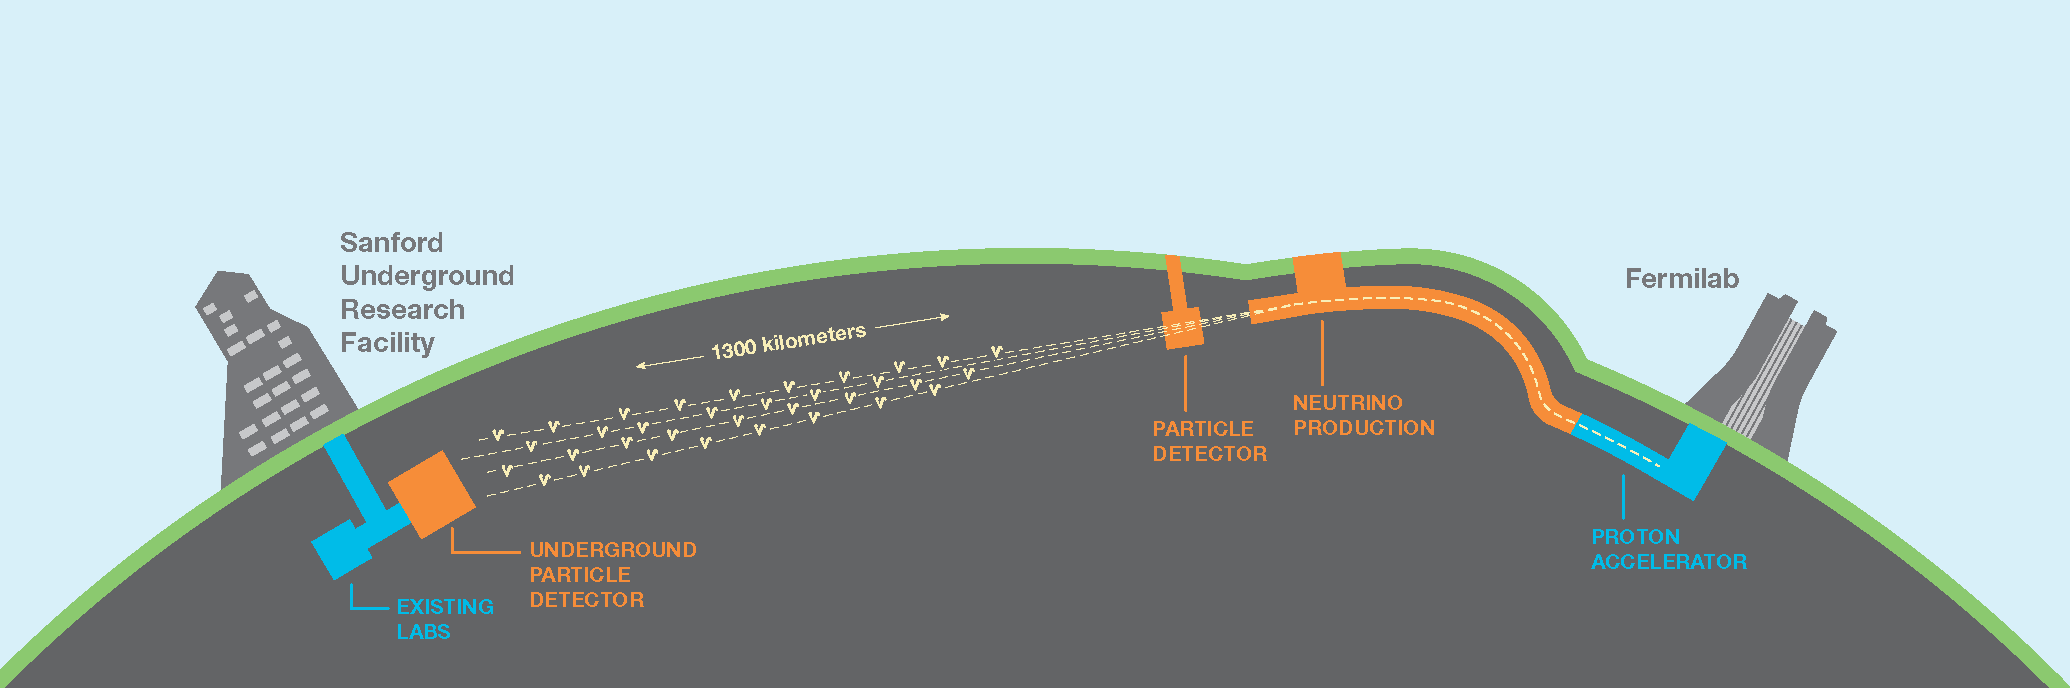
\includegraphics[width=\textwidth]{figures/dune_baseline.png}

	\caption
	[The Deep Underground Neutrino Experiment.]
	{The Deep Underground Neutrino Experiment. Figure from \cite{Abi:2020wmh}.}

	\label{fig:dune_baseline}

\end{figure}

The DUNE experiment will be a next generation neutrino physics and nucleon decay
experiment consisting of three principal components; an intense broad band 
neutrino beam and precise near detector based at the Fermilab National 
Accelerator Laboratory near Chicago, and a far detector at Sanford Underground 
Research Facility in South Dakota, approximately 1300 km away from the 
neutrino source, as demonstrated in Figure \ref{fig:dune_baseline}. The DUNE 
experiment identifies three primary scientific goals 
\cite{Abi:2020evt}:
\begin{itemize}
	\item Perform a comprehensive programme of neutrino oscillation measurements
		including measurements of \dcp{}, neutrino mass ordering, and the
		$\theta_{23}$ octant.
	\item Search for proton decay in several decay modes.
	\item Measure $\nu_e$ from a core--collapse supernova if one occurs within our
		galaxy during the lifetime of the experiment.
\end{itemize}
In addition, the experiment hopes to fulfill a significant programme of
secondary science goals:
\begin{itemize}
	\item Other accelerator based neutrino physics, such as non--standard
		interactions, sterile neutrinos, and CPT violation.
	\item Measurements of neutrino properties using atmospheric neutrinos.
	\item Dark matter searches in both the near and far detectors.
	\item A programme of neutrino interaction physics studies in the DUNE near
		detector.
\end{itemize}

To achieve these goals DUNE has opted to base the near and far detector designs
on the liquid argon time projection chamber (LArTPC) technology. The DUNE
far detector will consist of four LArTPC detectors each with 10 kt of active
liquid argon mass. This technology will have never before been used on this
scale, and therefore, there has been a significant programme of LArTPC research
and development ongoing to validate and characterise the performance of the 
technology for DUNE. 

\subsection{Liquid Argon Time Projection Chambers}
A LArTPC consists of a large volume of highly--purified liquid argon immersed in
an electric field. Charged particles traversing the liquid argon produce two
primary energy depositions, a trail of ionisation electrons along their path,
and prompt ultra--violet scintillation photons. After deposition the ionisation
electrons drift in the electric field toward the charge readout plane where they
induce electrical signals. Liquid argon is transparent to its own scintillation
light and therefore the scintillation photons can travel through the argon to be
collected in a photon detection system.The LArTPC detection principal is 
illustrated in Figure \ref{fig:lartpc}. 

\begin{figure}

	\centering

	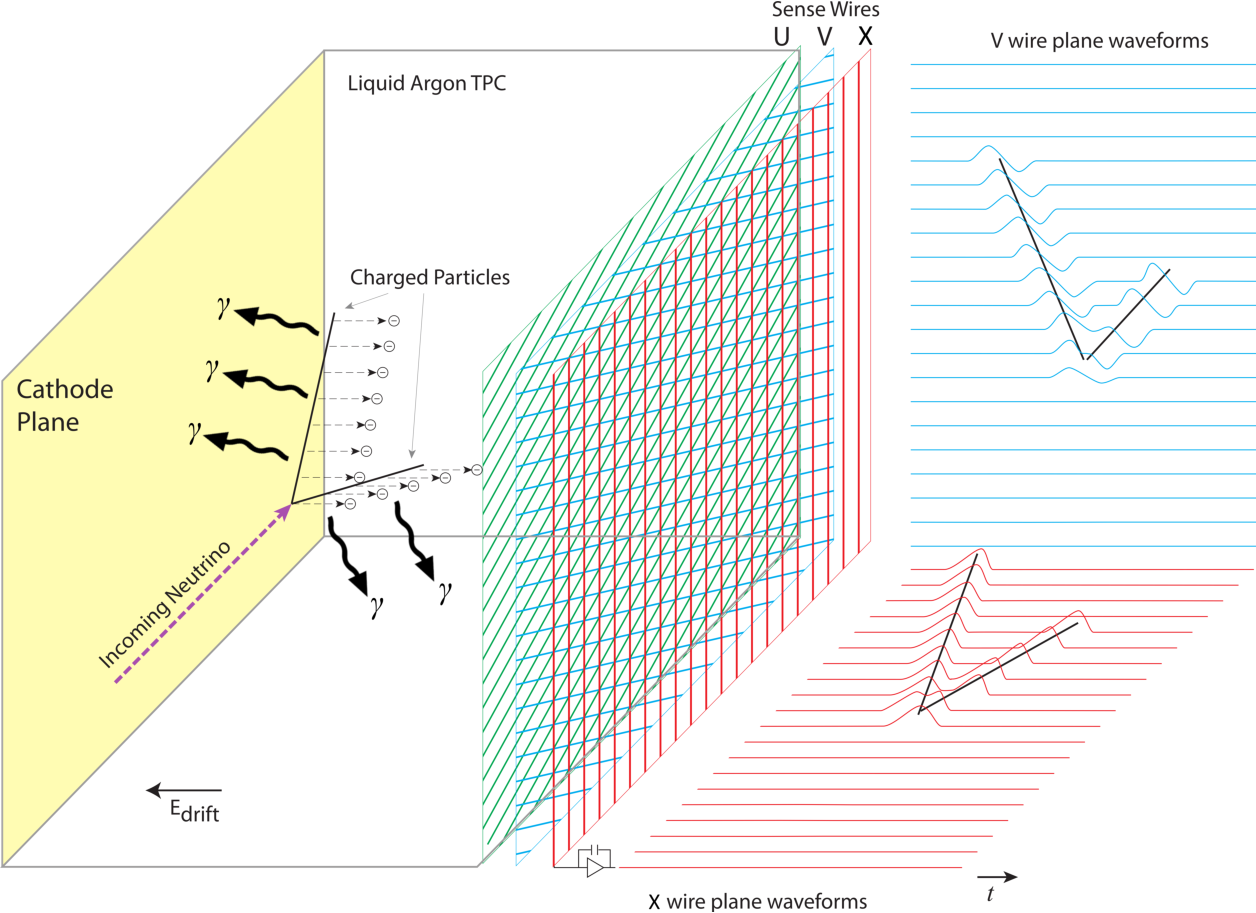
\includegraphics[width=\textwidth]{figures/LArTPC_Concept.pdf}

	\caption
	[LArTPC detection principal.]
	{LArTPC detection principal. Figure from \cite{Abi:2020loh}.}

	\label{fig:lartpc}

\end{figure}

\subsubsection*{The Role of Light in LArTPCs}

The ionisation signals in a LArTPC are slow, it takes charge milliseconds to
travel from the cathode plane to the anode plane. In contrast, scintillation 
photons only take on the order of nanoseconds to reach the closest anode 
plane. This scintillation light plays an important role in the accurate 3D 
reconstruction of interactions in the LArTPC, it provides a $t_0$. 

In a LArTPC interactions play out much quicker than the detector is able to 
record them; as such each event actually integrates over a large number of
interactions within the readout window, analogous to taking a photograph with a 
long exposure. The true time, $t_0$, of the interactions in the event cannot be 
reconstructed from the ionisation signals alone; by utilising the much faster 
scintillation signals the time of interactions can be calculated with much 
higher precision, this data can then be used to correct the position offset
caused in the ionisation signals.

\bigskip

The details of the charge readout and photon detection systems are specific to 
each detector, but broadly speaking LArTPC detectors can be split into two 
main categories: single--phase and dual--phase. In a single--phase detector the
drifting ionisation electrons remain in the liquid argon and the signals are 
typically read out on three anode wire planes. A dual--phase LArTPC contains an
additional region of gaseous argon in which a high electric field, known as the
extraction field, is applied to extract the ionisation from the liquid 
before it is amplified and collected on a pair of anode wire planes 
\cite{Abi:2020wmh}.

\bigskip

\protodune{} is one of two large scale prototypes for the DUNE far detector
modules, which focusses on the single--phase LArTPC technology. The DUNE far
detector modules feature a modular design in which each module is built up of a
number of identical components, \protodune{} was designed to prototype the
design of many of these components at a 1:1 scale, including the anode planes,
cathode plane, and photon detectors. The \protodune{} experiment has four 
primary goals, as outlined in the Technical Design Report \cite{Abi2017}:
\begin{itemize}
	\item Prototype the production and installation procedures for the
		single--phase far detector design.
	\item Validate the design from the perspective of basic detector performance;
		this can be achieved with cosmic-ray data. 
	\item Accumulate large samples of test-beam data to understand/calibrate the
		response of the detector to different particle species.
	\item Demonstrate the long-term operational stability of the detector as part
		of the risk mitigation program ahead of the construction of the first 10 kt
		far detector module.
\end{itemize}
As such, \protodune{} represents a significant milestone in the development of
the far detector for the DUNE experiment. Its successful operation, both in a 
test beam and with cosmic rays, provides valuable data with which to understand
reconstruction and analysis of the data that will be collected by the DUNE far 
detector.

\section{The \protodune{} Detector} \label{sec:pdsp_detector}

The \protodune{} detector is located at the Neutrino Platform at CERN along the
H4 beamline. It is a single--phase LArTPC detector with a total liquid argon 
mass of 0.77 kt, making it the largest monolithic single--phase liquid argon TPC
to be built to date. The TPC comprises the following major components, which 
are illustrated in Figure \ref{fig:pdsp_tpc}:
\begin{itemize}
	\item A cathode plane constructed of modular Cathode Plane Assemblies (CPA).
	\item Two anode planes constructed of modular Anode Plane Assemblies (APA).
	\item A photon detection system (PDS) which is integrated into the APAs.
	\item A field cage (FC), beam plug, and high voltage systems (HV).
	\item Readout electronics and Data Acquisition System (DAQ).
\end{itemize}
The detector components are designed to be an almost exact replica of the final 
single--phase far detector modules, but the detector has an overall scaling 
factor of approximately $1:20$ in terms of total liquid argon mass 
\cite{Abi2017}.

\begin{figure}

	\centering

	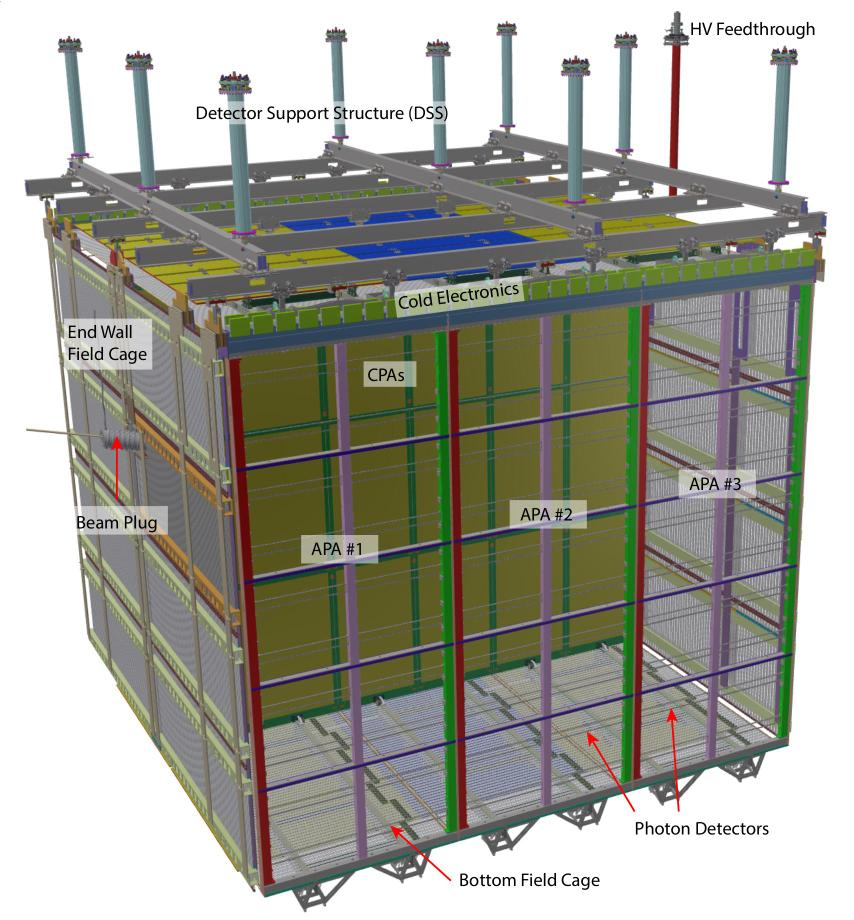
\includegraphics[width=0.9\textwidth]{figures/pdsp_tpc.jpg}

	\caption
	[The main components of the \protodune{} TPC.]
	{The main components of the \protodune{} TPC. Figure from \cite{Abi2017}.}

	\label{fig:pdsp_tpc}

\end{figure}

\subsection{The Liquid Argon TPC}

The \protodune{} TPC has an active volume of 6 m (height) $\times$ 7.2 m (width,
drift direction) $\times$ 7 m (length, approximate beam direction). The cathode 
plane at the center of the active width is flanked by two anode planes which 
define two 3.6 m drift volumes. The field cage around these two drift volumes
helps to ensure a uniform electric field within the drift region.

Each anode plane is modularly constructed from three APAs which have dimensions
6 m (height) $\times$ 2.3 m (width). The APA frame holds three sets of parallel
wires on the inward and outward facing sides, these are oriented at different 
angles to enable 3D reconstruction. The outer two sets of wires are induction
wires, these are electrically connected and biased such that they are
electrically transparent to the drifting ionisation; ionisation passing the
induction wires causes an induced bi--polar signal. The third set of wires are 
known as collection wires, they are not electrically connected; when drifting 
ionisation approaches the collection wires it is absorbed producing a 
uni--polar signal. In \protodune{} each set of induction wires contains 800
wires at a 4.67 mm spacing, and each set of collection wires contains 480 
wires at a 4.79 mm spacing. 

The wire planes from each APA are read out by electronics mounted on the APA 
frame; these electronics are submerged in the liquid argon and therefore 
referred to as cold electronics (CE). A total of 2560 electronics channels are 
used to read out the data from each APA. The CE amplify, shape, and digitise the
signals from the wires before transmitting them outside the TPC to the Warm
Interface Boards (WIB). The WIBs collate the data from the CE boards along with
timing information from the timing system and pass the data onto the 
Data Acquisition System (DAQ).

The cathode plane in \protodune{} consists of an array of 18 CPA modules, 2 m 
(height) $\times$ 1.2 m (width). The cathode plane is held at -180 kV to 
provide a 500 $\mbox{V/cm}$ drift field in each of the drift volumes. The 
field cage surrounding the drift regions ensures that the electric field is 
uniform across the detector volume by providing the necessary electrical
boundary conditions.

One area in which the design of \protodune{} differs from the far detector is
the inclusion of the beam plug. This is necessary to minimize interactions
between the charged particle test beam and the cryostat before the beam enters 
the active region of the detector. A cylindrical beam plug, containing 
nitrogen gas, penetrates from the cryostat wall into the field cage at 
location of the incoming test beam. 

\subsection{The Photon Detection System}

The PDS in \protodune{} is integrated into the APAs. Ten photon detector modules
are embedded in each APA frame between the layers of wires on each APA 
face, as shown in Figure \ref{fig:pdsp_tpc}. Three types of photon detector
module were tested in \protodune{}, two very similar module designs based on
coupling silicon photomultipliers to wavelength shifting bars, and a third 
novel design know as the ARAPUCA light trap. The operating principles of the 
two designs are illustrated in Figure \ref{fig:pdsp_pd}.

\begin{figure}

	\centering

	\begin{subfigure}[b]{0.28\textwidth}
		\centering
		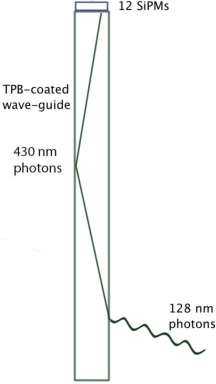
\includegraphics[height=0.3\textheight]{figures/pdsp_pd.pdf}
		\caption{Waveguide.}
		\label{fig:pd_bars}
	\end{subfigure}
	\hfill
	\begin{subfigure}[b]{0.67\textwidth}
		\centering
		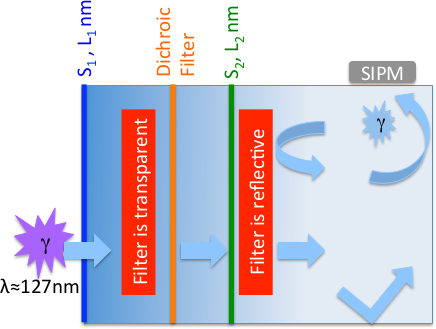
\includegraphics[height=0.3\textheight]{figures/pdsp_arapuca.png}
		\caption{ARAPUCA.}
		\label{fig:arapuca}
	\end{subfigure}

	\caption
	[The operating principal of the photon detector modules in \protodune{}.]
	{The operating principal of the photon detector modules in \protodune{}.
	Figure \subref{fig:pd_bars} from \cite{Abi2017}. Figure \subref{fig:arapuca} 
	from \cite{Machado:2016jqe}}

	\label{fig:pdsp_pd}

\end{figure}

The majority of the photon detector modules in \protodune{} consist of 
wavelength shifting bars coupled to silicon photomultipliers (SiPM). 
Tetraphenyl-butadiene (TPB) is used to shift the wavelength of the light 
from ultra--violet to blue before the light is transmitted down the waveguide to
the SiPMs. The main difference between the two nominal designs is in the 
wavelength of transmission within the waveguide; in one case the wavelength is 
transmitted at the blue wavelength produced by the TPB, in the other case the 
blue light from the TPB is first absorbed in the waveguide which then produces 
green light which is transmitted down the waveguide.

A small number of the photon detector modules in \protodune{} feature a novel 
design known as an ARAPUCA light trap. In this design the photons are trapped 
in a small box through a sequence of wavelength shifting and optical 
filtering, significantly increasing the photon detection efficiency 
\cite{Segreto:2018jdx}. An ARAPUCA light trap consists of a 5 cm $\times$ 5 cm 
$\times$ 1 cm box which is coated with a highly reflective surface, on one 
side of the box is the filtering window, and on the other a SiPM. Incoming 
ultra--violet photons are shifted to the blue spectrum before passing through 
a dichroic filter which has a tunable wavelength cut--off at which it 
transitions from being transparent to reflective. After passing through the 
filter the photons are shifted again, this time from blue to green, such that 
if they get back to the filter it is reflective. As such green photons can 
be trapped within the ARAPUCA until they come into contact with the SiPM, 
providing increased photon detection efficiency. Each ARAPUCA photon detector 
module in \protodune{} features an array of these traps arranged in a line 
across the width of an APA.

Unlike with the TPC electronics, there are no front--end electronics in the LAr
volume for the PDS, the unamplified analogue signals are transmitted out of the
cryostat before processing and digitisation. Each photon detector module has 
12 SiPMs which are read out in threes such that each module corresponds to 4 
readout channels. The 40 readout channels from each APA are processes by four 
so called SiPM Signal Processors (SSP), which handle 10 channels each and are 
mounted on the top of the cryostat. After processing in the SSPs the PDS data is
passed onto the DAQ along with the TPC data.

\section{The H4 beamline} \label{sec:h4}

The \protodune{} experiment is located at the end of the H4 beamline at CERN,
the location of the beamline with respect to the detector is illustrated in
Figure \ref{fig:pdsp_CRT}.  The beam can be configured to provide hadron, 
muon, and electron beams with energies in the range 1--7 GeV into the 
detector. 

The H4 beamline is a tertiary beamline which is produced when a secondary beam
from the T2 primary target interacts with a secondary target. Particles from the
secondary beam are selected based on momentum and charge before travelling down
the H4 beamline to \protodune{}. A schematic of the beamline instrumentation
(BI) and magnets in the H4 beamline is given in Figure \ref{fig:h4_schem}. 

\begin{figure}

	\centering

	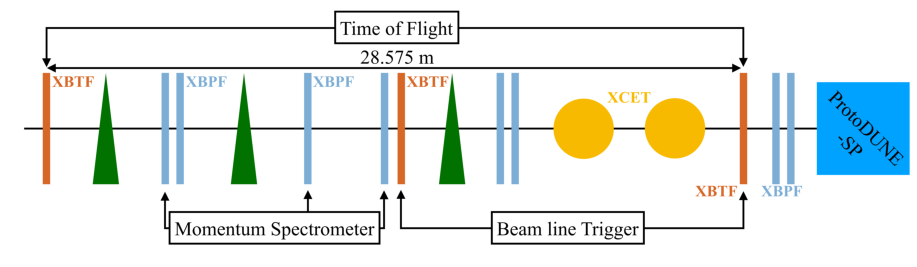
\includegraphics[width=\textwidth]{figures/h4_schem.pdf}

	\caption
	[Schematic of the H4 beamline magnets and instrumentation.]
	{Schematic of the H4 beamline magnets and instrumentation. Figure from
	\cite{protoduneperf}.}

	\label{fig:h4_schem}

\end{figure}

By combining momentum measurements from the profile monitors with time of flight
(TOF) and Cerenkov measurements the beam momentum and composition can be 
measured. The predicted and measured distribution of TOF vs momentum for data 
from a number of runs at different momenta is shown in Figure \ref{fig:h4_tof}.
This information is used to trigger the detector during beam running, and is
sent to the central trigger board for distribution to the detector components.

\begin{figure}

	\centering

	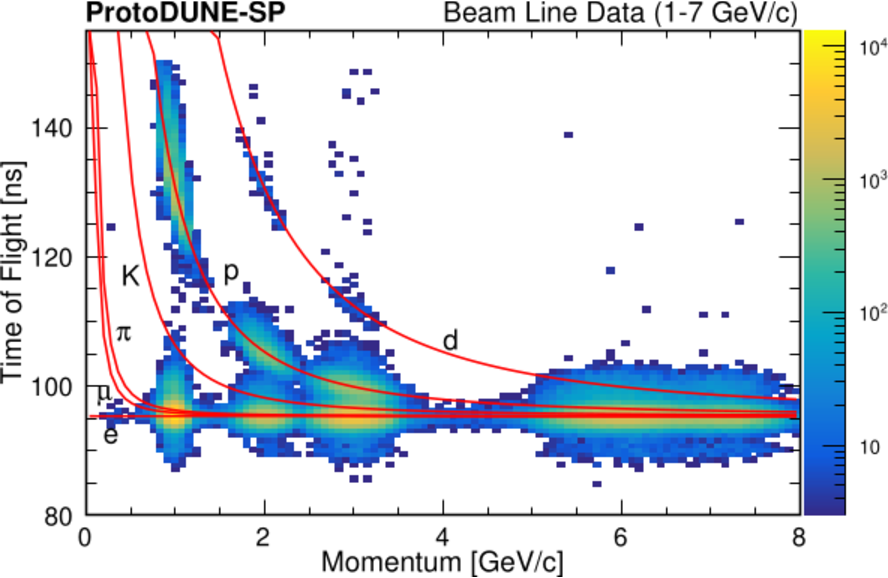
\includegraphics[width=\textwidth]{figures/h4_tof.pdf}

	\caption
	[Time of flight vs momentum distributions from the H4 beamline
	instrumentation.]
	{Time of flight vs momentum distributions from the H4 beamline
	instrumentation. Figure from \cite{protoduneperf}}

	\label{fig:h4_tof}

\end{figure}

\section{The Cosmic Ray Tagger} \label{sec:pdsp_cosmic}

As a surface level detector with no overburden \protodune{} measures a
significant rate, on the order of 20 kHz, of cosmic ray muons, corresponding 
to an average of 60 muons per 3 ms readout window. These muons provide a 
useful source of calibration data in to form of long tracks and stopping muons. 
The Cosmic Ray Tagger (CRT) in \protodune{} was installed on the upstream and
downstream faces of the TPC to trigger the detector for cosmic--ray muons which
travel parallel to the anode plane. In addition the CRT provides an additional
source of $t_0$ tagged tracks for calibration.

The CRT consists of four parts, two upstream assemblies and two downstream
assemblies, the locations of the CRT assemblies is illustrated in Figure
\ref{fig:pdsp_CRT}. Each CRT assembly is constructed from overlapping 
scintillation counters which cover an area 6.8 m high and 3.65 m wide. 
Scintillation strips of length 365 cm and width 5 cm are placed in 
perpendicular arrays to give two--dimensional reconstruction within each CRT 
assembly. By combining data from upstream and downstream CRT assemblies with a 
time coincidence requirement the trajectories of tracks can be reconstructed.

\begin{figure}

	\centering

	\begin{subfigure}[b]{\textwidth}
		\centering
		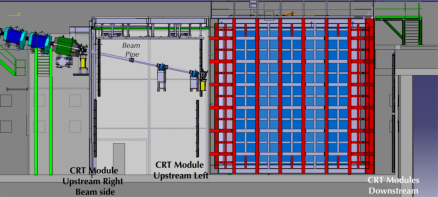
\includegraphics[width=0.6\textwidth]{figures/crt_side.pdf}
		\label{fig:crt_side}
		\caption{Side view.}
	\end{subfigure}

	\vspace{3mm}

	\begin{subfigure}[b]{\textwidth}
		\centering
		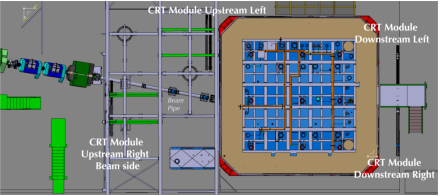
\includegraphics[width=0.6\textwidth]{figures/crt_top.pdf}
		\label{fig:crt_top}
		\caption{Top view.}
	\end{subfigure}

	\caption
	[Location of the H4 beamline and cosmic ray taggers in relation to the
	\protodune{} detector.]
	{Location of the H4 beamline and cosmic ray taggers in relation to the
	\protodune{} detector. Figures from \cite{protoduneperf}.}

	\label{fig:pdsp_CRT}

\end{figure}

\section{The Data Acquisition System}

Data from the TPC, PDS, and CRT in \protodune{} are collated by the Data 
Acquisition system (DAQ). The DAQ distributes triggers, compresses and packages 
the data into events, monitors the data quality, and stores the data ready for 
future analysis. An overview of the \protodune{} DAQ system is seen in Figure 
\ref{fig:pdsp_daq}; there are four primary data flows in the system: TPC, PDS,
CRT, and BI. Timing and triggering signals are distributed to the detector 
components by the timing board which maintains a 50 MHz clock and receives 
$\sim 40 \mbox{Hz}$ of triggers from the Central Trigger Board (CTB) based on 
data from the BI and CRT \cite{Abi2017}.

\begin{figure}

	\centering

	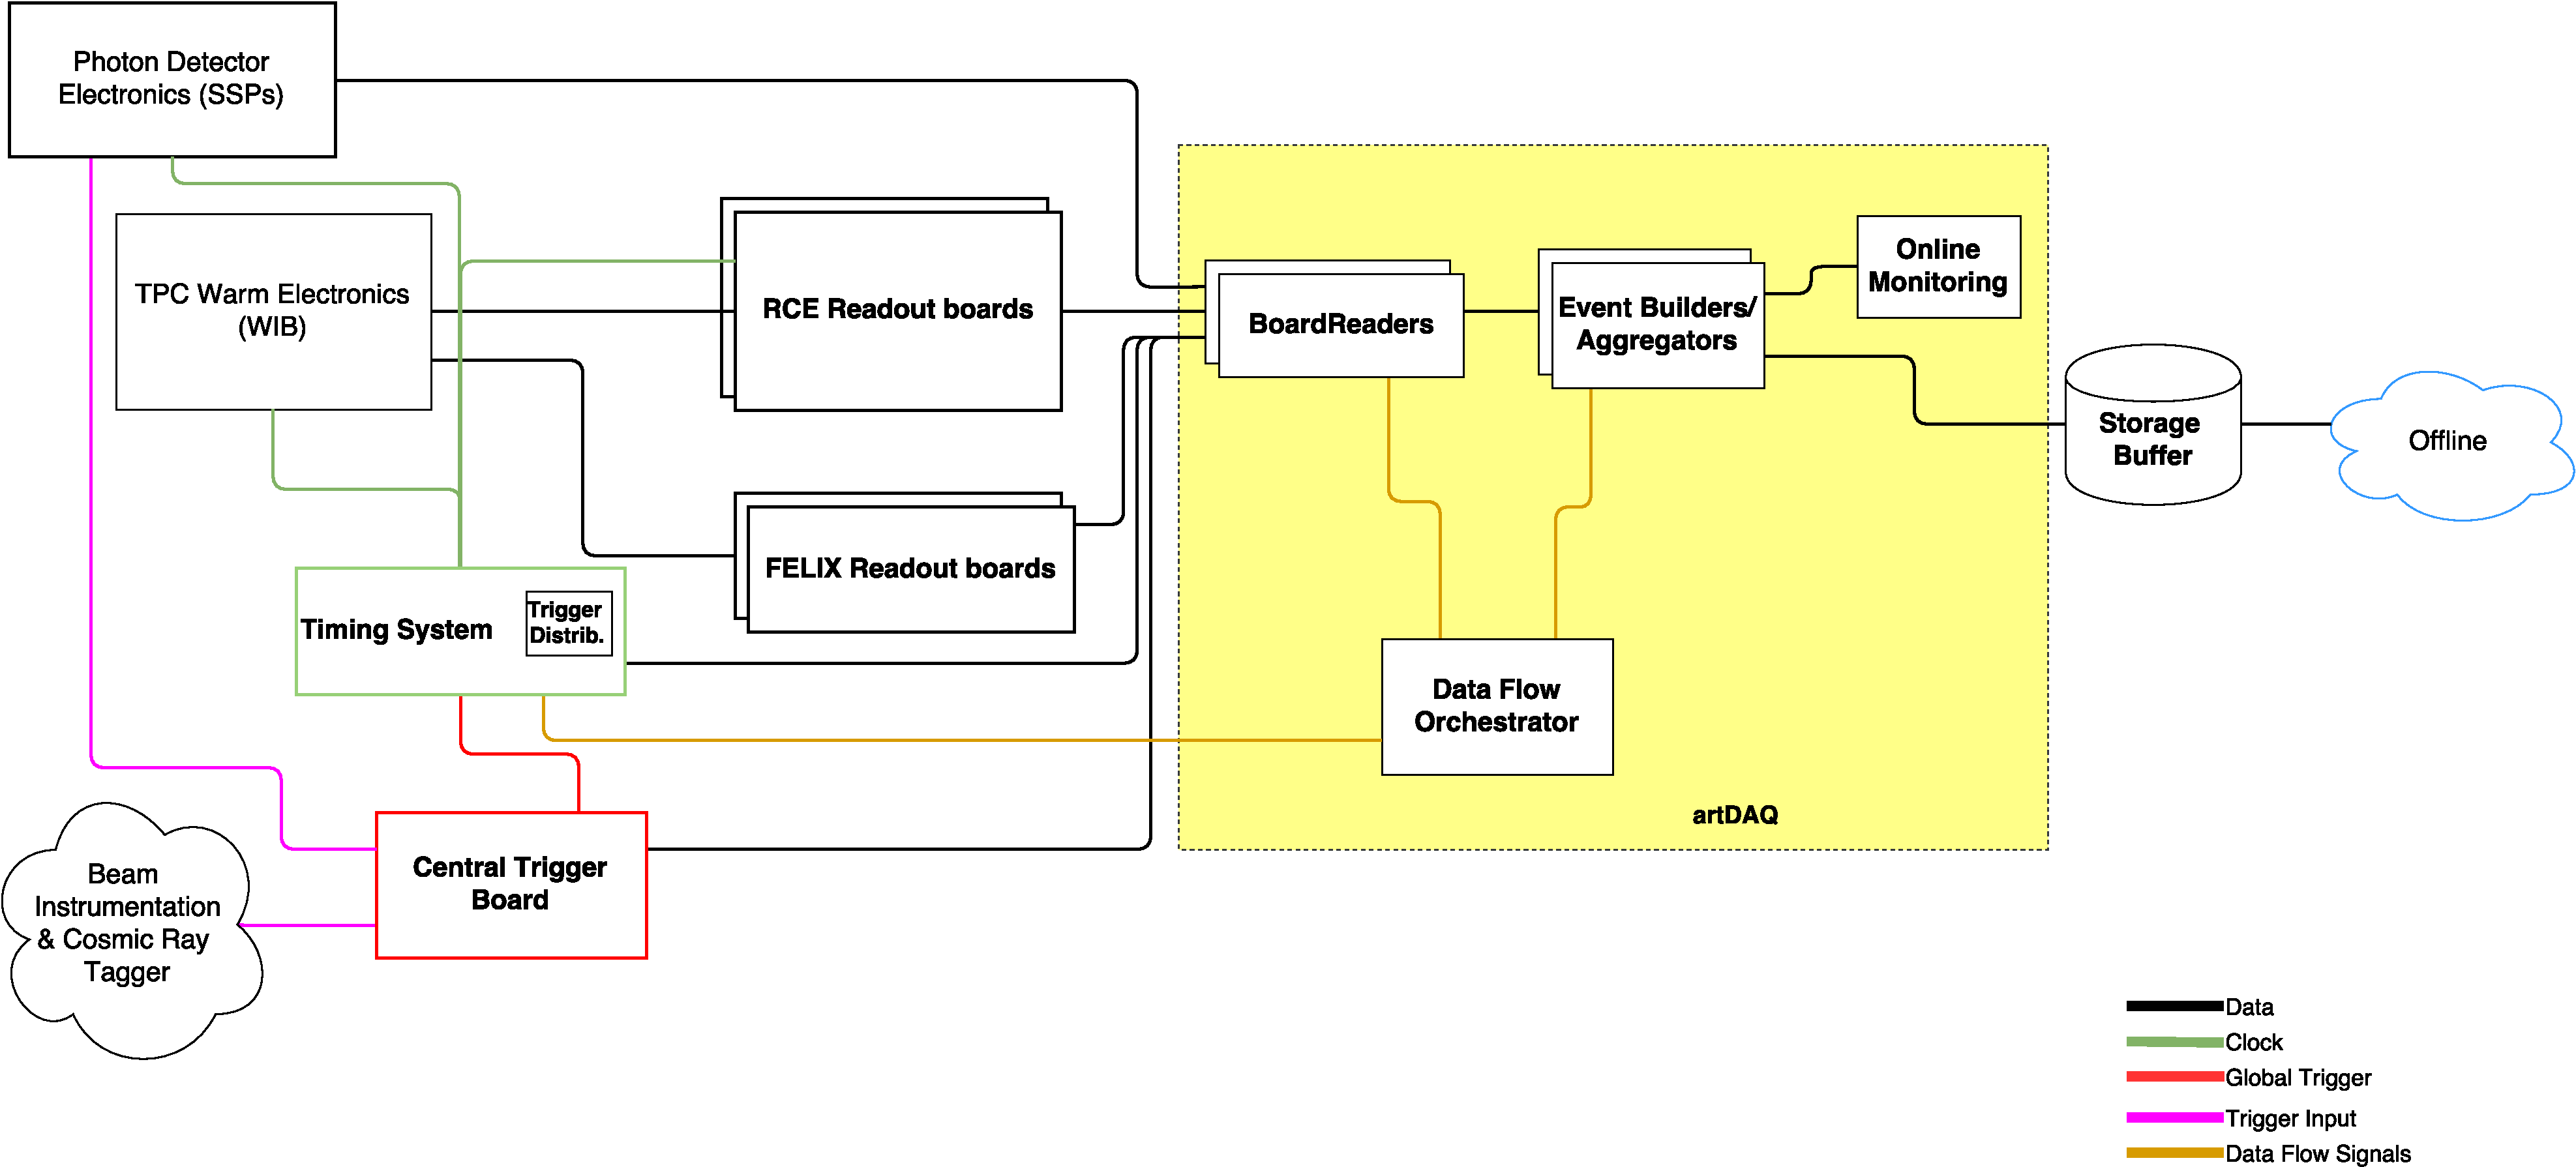
\includegraphics[width=\textwidth]{figures/pdsp_daq.pdf}

	\caption
	[Outline of the data acquisition system in \protodune{}.]
	{Outline of the data acquisition system in \protodune{}. Figure from
	\cite{Abi2017}.}

	\label{fig:pdsp_daq}

\end{figure}

The \protodune{} TPC contains a total of 15,360 wires spread across the six
APAs, the wires are digitized at a rate of 2 MHz resulting in an overall data
flow of around 480 $\mbox{Gb/s}$ from the TPC electronics. An event in
\protudune{} corresponds to a continuous readout of the detector for 3 ms,
resulting in 6000 samples from each wire; data is buffered such that the readout
window can be opened 250 $\mu$s before the trigger time. Data from the TPC is
received by two systems, a system based on Reconfigurable Computing Elements
(RCE) \cite{7431254} handles the data from five APAs while data from the sixth 
is received by a system based on Front--End Link Exchange (FELIX) cards which 
have been developed by the ATLAS collaboration \cite{Anderson_2016}.

The software layer of the \protodune{} DAQ is based on Fermilab's artdaq 
\cite{6495515}. This component is primarily responsible for acquiring the data,
packaging it, and storing it locally. Triggered events are queued and 
distributed to the board readers and event builders by the Data Flow 
Orchestrator. There are multiple board readers which are each responsible for 
processing the data from specific hardware components, details vary between 
specific board readers but generally these processes are responsible for 
formatting the data from each component ready for aggregation. Data from the
various detector components are aggregated by the event builders, which are
responsible for assembling the completed events. After compression events have
an average size of 60 MB. Artdaq is also responsible for the real--time 
monitoring of data quality via the online monitoring system, this system will be
discussed in Section \ref{sec:pdsp_om}.

\section{Simulation} \label{sec:simulation}

Simulation and reconstruction of \protodune{} data takes place in the LArSoft
framework \cite{Snider2017}. LArSoft is a software suite for simulating and
reconstructing data collected by LArTPC detectors based on the art event 
framework from Fermilab \cite{Green:2012gv}. LArSoft is under active use and
development by a number of participating LArTPC based experiments, with each
experiment making use of its core functionality as well as experiment specific
code. The simulation and reconstruction of \protodune{} data in the LArSoft
framework will be discussed in sections \ref{sec:simulation} and
\ref{sec:reconstruction} respectively.

Simulation in LArSoft is broken down into three sequential stages: generation,
propagation, and detector simulation. The initial state particles are produced
in the generation step, the propagation and interaction of these particles in
the detector is simulated during the propagation step, finally the transport of 
energy depositions and simulation of detector effects are handled by the
detector simulation phase.

As a surface based detector in a test beam, \protodune{} is subject to three
main sources of particles: beam particles, beam halo particles, and cosmic ray
particles. The beam particle and beam halo flux in the vicinity of 
\protodune{} was provided by simulations of the H4 beamline 
\cite{Booth:2019brj} based on two simulation frameworks, G4beamline 
\cite{g4beamline} and FLUKA \cite{BOHLEN2014211}. The cosmic ray flux in
\protodune{} is simulated using CORSIKA \cite{Heck:1998vt}. Finally, low energy 
radiological backgrounds in LAr are simulated, these include $^{39}\mbox{Ar,} ^
{85}\mbox{Kr, and } ^{222}\mbox{Rn}$.

After generation, the particles are allowed to propagate and interact in the 
detector geometry, including the cryostat, external systems, and experimental
hall. This is simulated using GEANT4 \cite{Agostinelli:2002hh} which tracks 
particles in small steps; the step size, $300 \mu m$, is chosen to be much 
smaller then the spatial resolution of the detector to allow for small--scale 
processes like showering to be accurately simulated. 

Particles which propagate through the detector during the propagation phase of
the simulation leave energy deposits in the form of ionisation electrons and
scintillation photons. It takes 23.6 eV to ionise a single argon atom and 
around 19.5 eV to produce a single scintillation photon, as such a 
minimum--ionising particle (MIP), which deposits around $2 \mbox{MeV/cm}$ 
in liquid argon, will produce tens of thousands of electrons and photons per cm.

The detector simulation phase of the simulation chain is responsible for
drifting the ionisation electrons towards the collection wires, propagating the
simulated photons to the photon detectors, and simulating the response of the
wires, SiPMs, and electronics to the signals. The shear number of ionisation 
electrons and scintillation photons produced in a \protodune{} event makes 
simulating the propagation of the full set of particles impractical and 
therefore LArSoft employs approximation techniques to accurately predict the 
observed signals within a reasonable computation time. A number of detector 
effects are taken into account when simulating the electron drift: 
electron--ion recombination, transverse and longitudinal diffusion, electric 
field distortions due to space charge, and electron capture on impurities. 

When the ionisation and scintillation signals arrive at the detector components,
simulated waveforms are produced based on the induced signals produced in the
detector components. These signals are converted into electrical signals
by electronics simulation which is completed in LArSoft. The electronics 
simulation includes simulation of: electronics gain, noise, and analogue to 
digital conversion. The simulated waveforms produced by the \protodune{} 
simulation are then compressed and stored ready for reconstruction.

\section{Reconstruction} \label{sec:reconstruction}

% \subsection{Optical Reconstruction} \label{sec:op_reco}
% \mccorrect{TODO.}
% \subsection{TPC Reconstruction} \label{sec:tpc_reco}

An event consists of a synchronised set of waveforms from all of the TPC 
channels, with each event corresponding to 3 ms or 6000 samples. The particle
interactions within each event are reconstructed into objects like tracks and
showers which can be used for physics analyses, this sections provides a brief 
summary of the steps involved in this reconstruction.

First, the TPC waveforms are passed through a set of filtering algorithms which
are designed to reduce the noise on the waveforms, as well as to mitigate 
electronics effects such as sticky--codes and undershooting. An additional step
known as a 2D deconvolution is applied to extract the original signal from the
measured signal given a detector response function for the wire in question as
well as neighboring wires, this method has been described in detail by the 
MicroBooNE collaboration \cite{Adams:2018dra}. An example of the noise filtering
and 2D deconvolution techniques applied to a 7 GeV test beam event in 
\protodune{} data is given in Figure \ref{fig:2d_deconv}.

\begin{figure}

	\centering

	\begin{subfigure}{0.48\textwidth}
		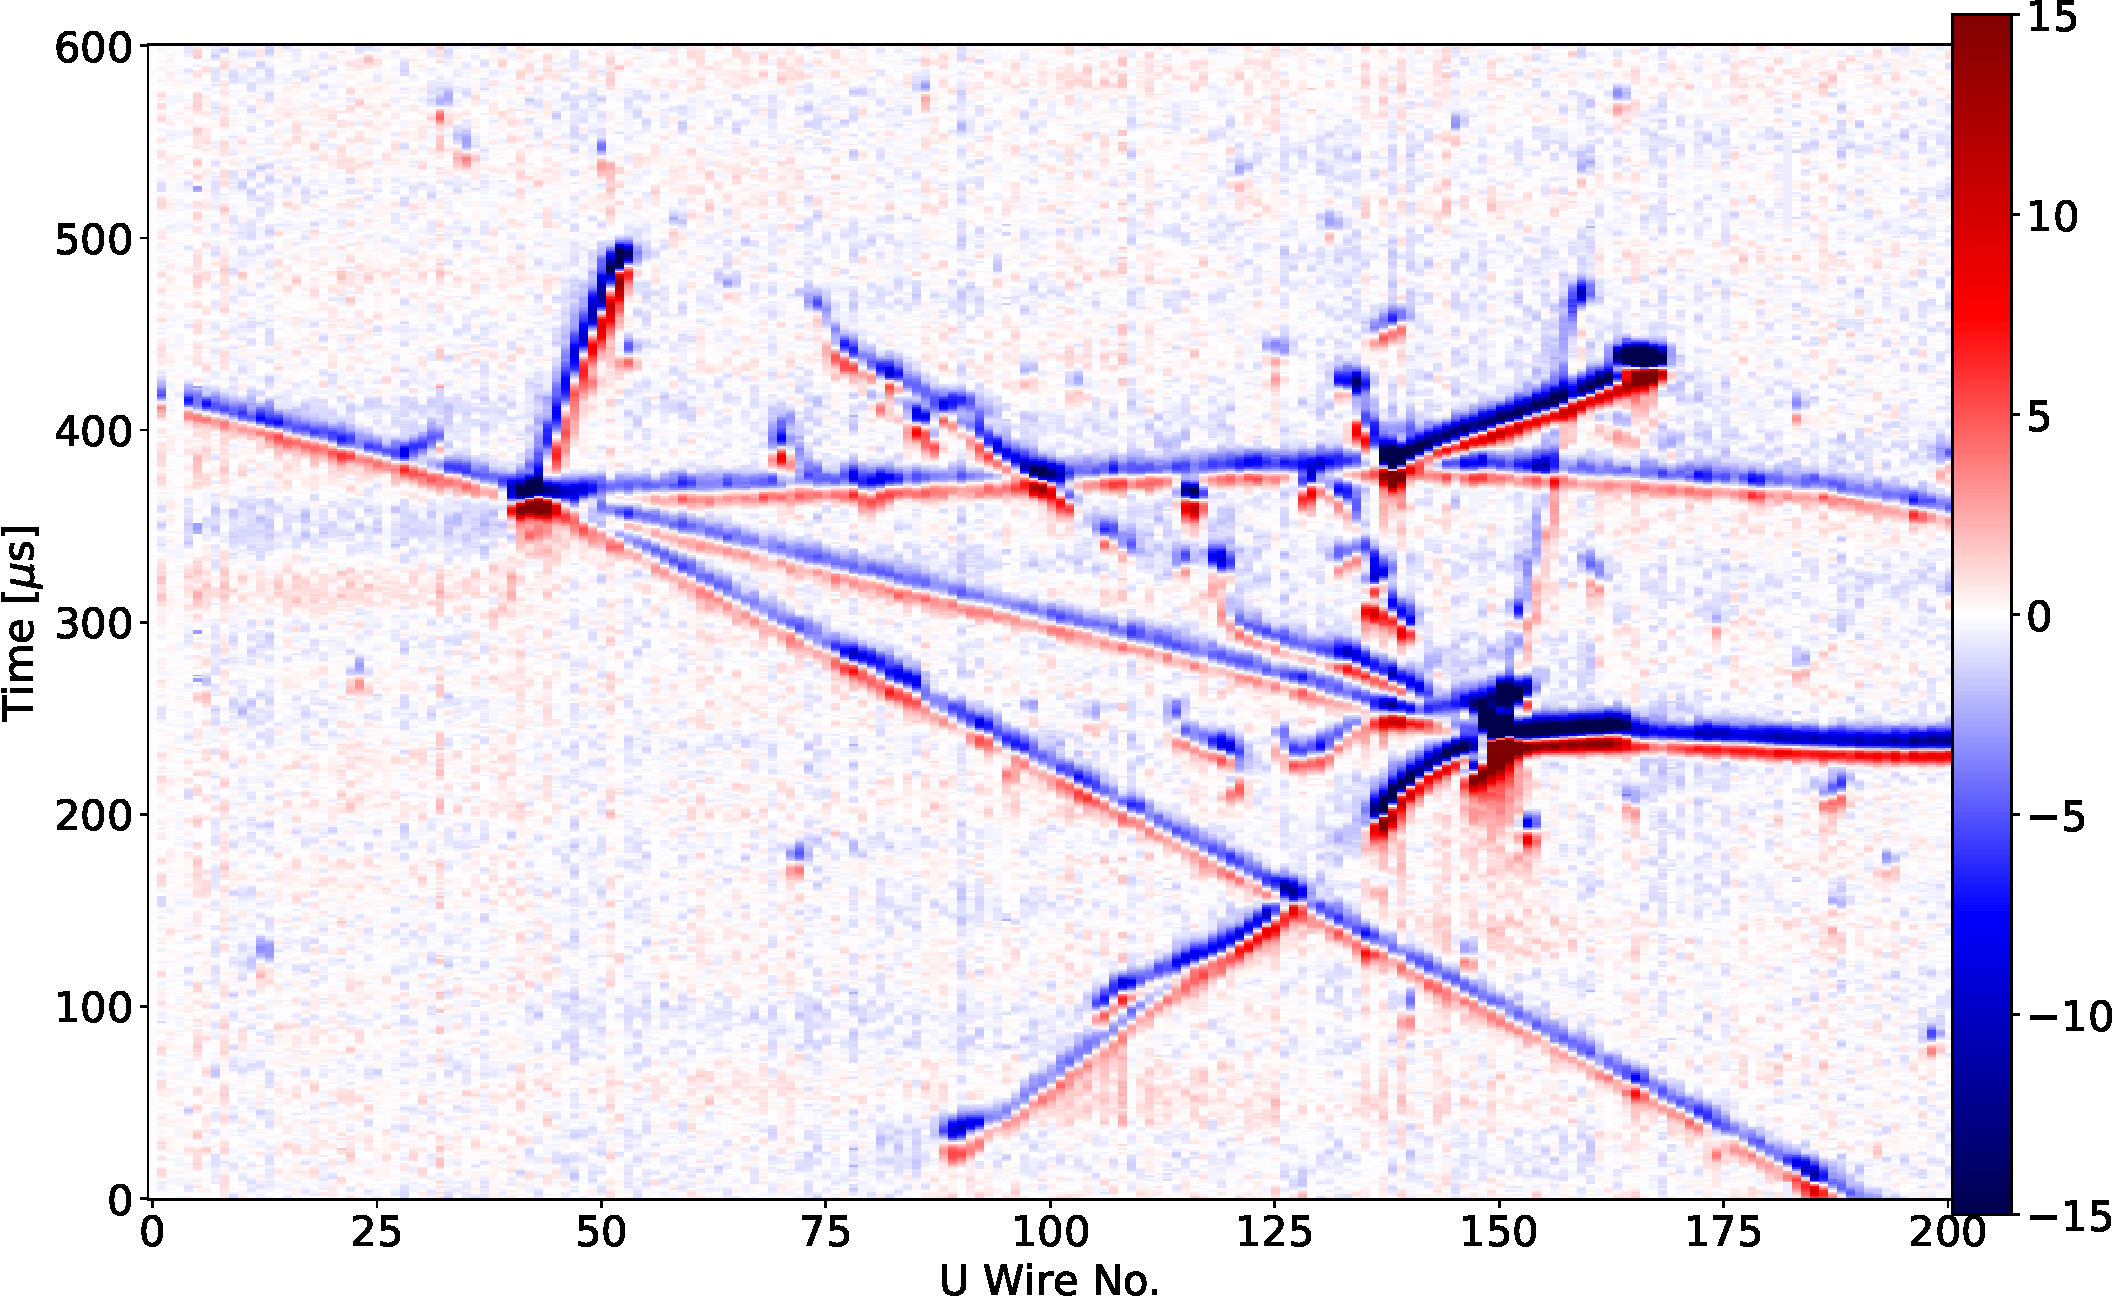
\includegraphics[width=\textwidth]{figures/protodune_evd_orig.pdf}
		\label{fig:pdsp_raw}
		\caption{Before noise filtering.}
	\end{subfigure}
	\hfill
	\begin{subfigure}{0.48\textwidth}
		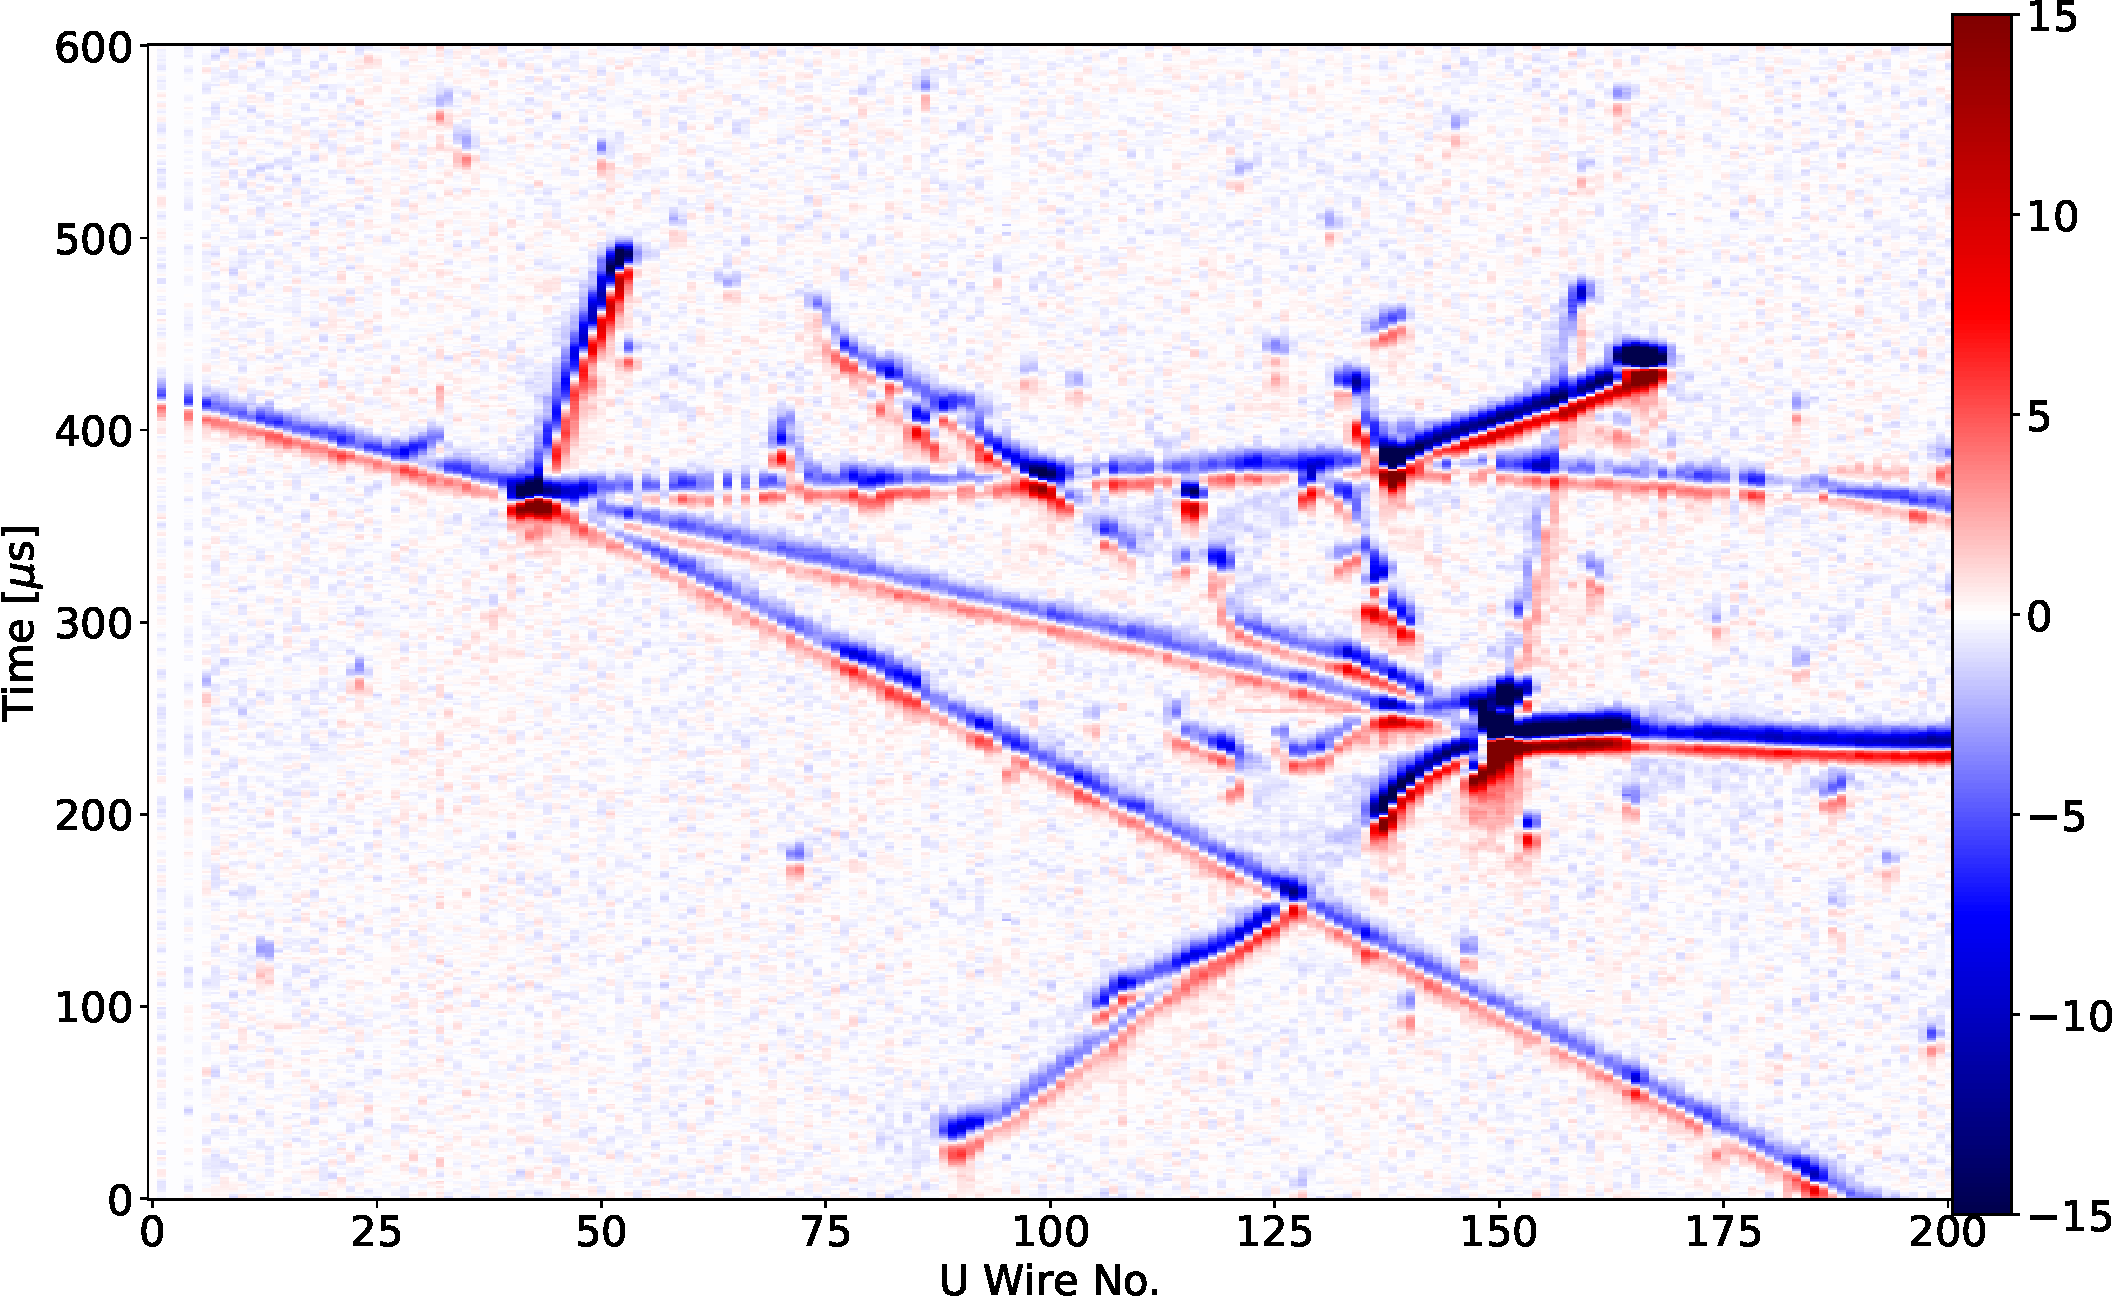
\includegraphics[width=\textwidth]{figures/protodune_evd_raw.pdf}
		\label{fig:pdsp_filt}
		\caption{After noise filtering.}
	\end{subfigure}
	\begin{subfigure}{0.48\textwidth}
		\vspace{5mm}
		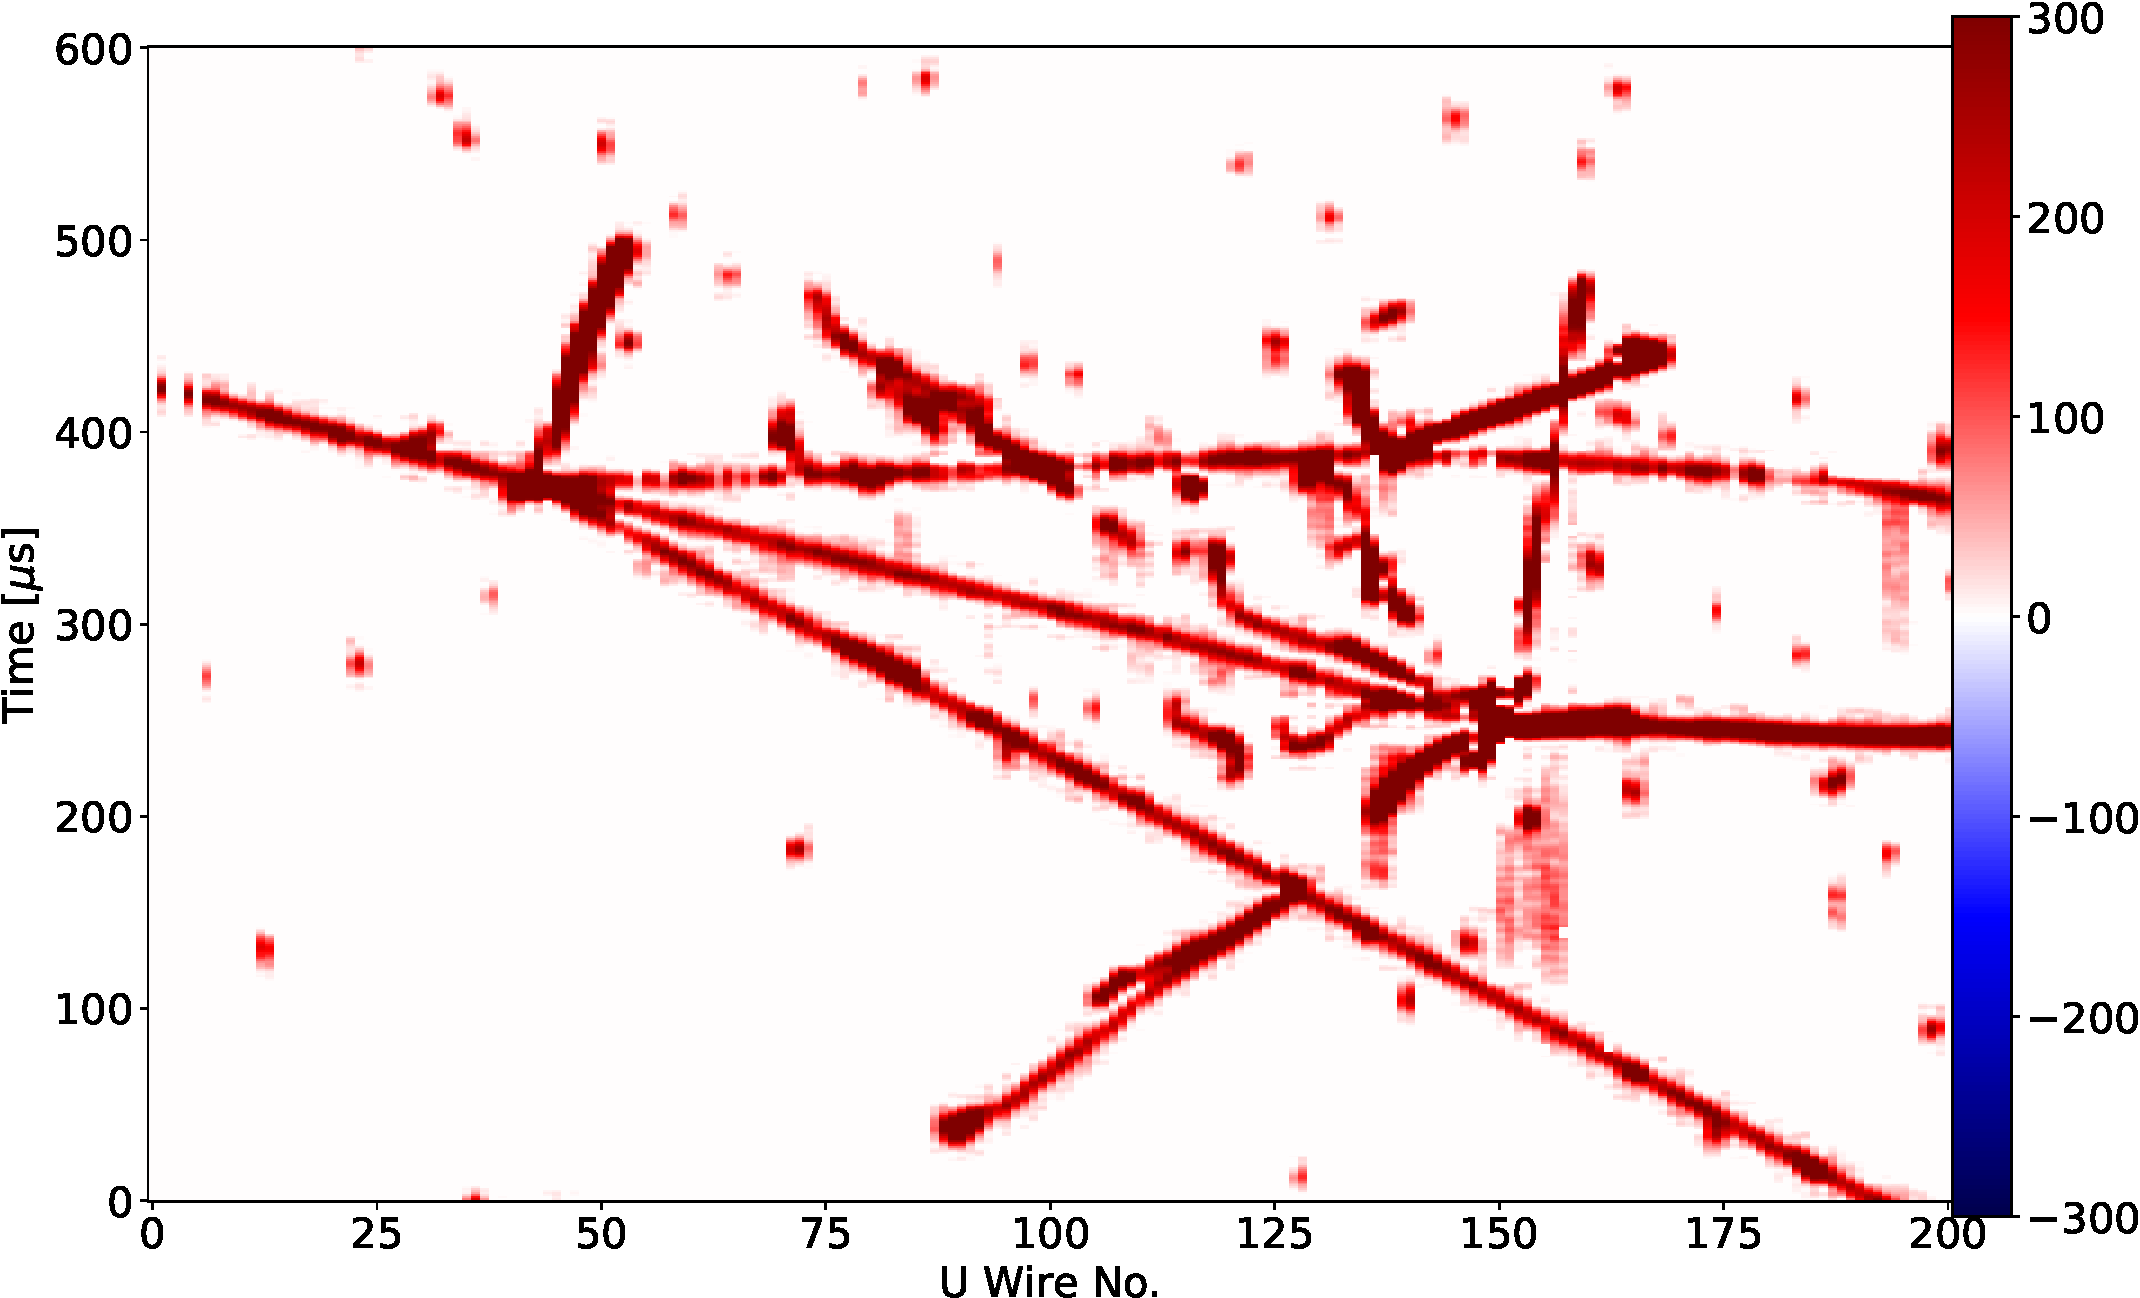
\includegraphics[width=\textwidth]{figures/protodune_evd_decon.pdf}
		\label{fig:pdsp_deconv}
		\caption{After 2D deconvolution.}
	\end{subfigure}

	\caption
	[Example of noise filtering and 2D deconvolution in \protodune{} data.]
	{Example of noise filtering and 2D deconvolution in \protodune{} data. Figures from \cite{protoduneperf}.}

	\label{fig:2d_deconv}

\end{figure}

Once the deconvoluted waveforms have been calculated, regions of interest (ROI) 
are defined, these are regions of high amplitude in which charge deposition is
likely to have occurred. Reconstructed hits are found within each region of
interest by fitting gaussian peaks to the peaks within the region; most hits
consist of a single gaussian peak, however in busy regions of the detector
multiple gaussian peaks may be used to fit a single pulse. Each reconstructed
hit will have an associated peak time, width, and integral, these objects form
the basic input for the subsequent pattern recognition algorithms. An example of
the reconstructed hits is shown in Figure \ref{fig:gaushit}.

\begin{figure}

	\centering

	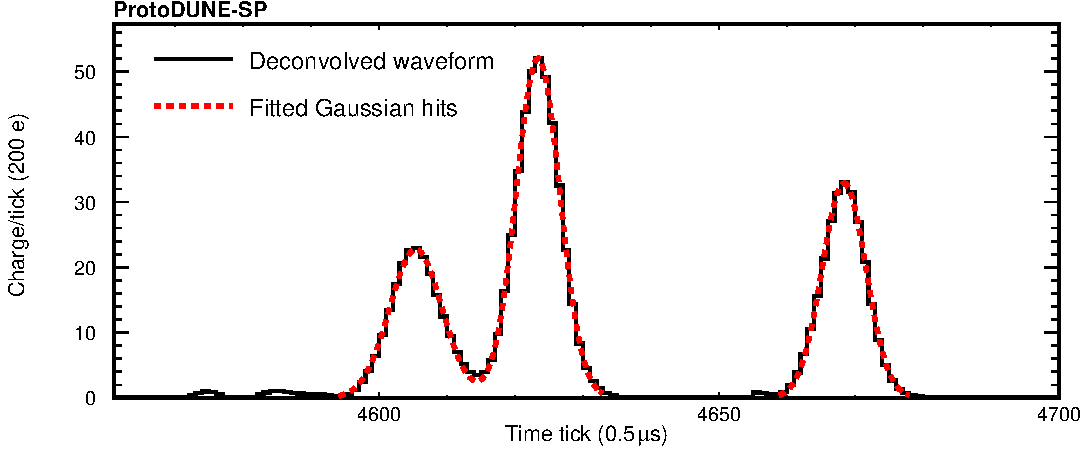
\includegraphics[width=\textwidth]{figures/gaushit.pdf}

	\caption
	[Reconstructed hits from \protodune{} data.]
	{Reconstructed hits from \protodune{} data. Figure from \cite{protoduneperf}.}

	\label{fig:gaushit}

\end{figure}

Pandora \cite{Marshall2015} is the primary pattern recognition software used in
\protodune{}. It takes a multi--algorithm approach to reconstructing particle
interactions in the detector, and has been successfully used by other LArTPC
detectors, such as MicroBooNE \cite{Acciarri:2017hat}. Pandora handles the 
clustering of hits into 2D clusters, the matching of 2D clusters into 3D
clusters, as well as the reconstruction of 3D objects like tracks and 
showers. Ultimately Pandora returns a tree of reconstructed Particle Flow
Particles (PFParticles), each corresponding to a distinct track or shower, and 
connected through parent--daughter relationships which define the particle flow 
in the interaction. Pandora reconstruction proceeds in two stages: a cosmic 
pass and a beam pass. 

First the cosmic pass reconstructs the event with algorithms designed to 
reconstruct track--like particles. Track stitching algorithms can be used to
assign a $t_0$ to tracks during this stage; any track which crosses either a CPA
or APA will produce track segments on either side of the boundary, these
segments point in the same direction but will have been displaced from each 
other in the drift direction based on the arrival time of the corresponding 
particle. The $t_0$ for that track is equal to half the time shift required to 
realign the two segments into a continuous track. After the cosmic pass any 
clear cosmic--ray candidates are removed under the following conditions 
\cite{protoduneperf}:
\begin{itemize}
	\item The particle travels through both the top and bottom of the detector.
	\item The assigned $t_0$ is inconsistent with the beam time.
	\item If no $t_0$ assigned, try $t_0 = 0$. If any hits are reconstructed 
		with positions outside of the detector this track is inconsistent with the 
		beam time.
\end{itemize}

Beam particle reconstruction considers only the hits that were not removed by 
being labelled as clear cosmic--rays. These hits are formed into 3D slices which
contain all the hits from a single parent particle and it's daughters. The
slices are reconstructed under both the cosmic--ray and beam particle
hypothesis, and a boosted decision tree (BDT) is used to determine whether a 
given slice is consistent with being a beam particle. 

Under the beam particle hypothesis a more complex chain of algorithms is used to
reconstruct a given slice, these algorithms are capable of reconstructing the
particle hierarchies seen in the complex hadronic interactions from the
\protodune{} beam. These algorithms return the particle flow of the interactions
in the form of PFParticles as well as the reconstructed interaction vertex for
the primary beam particle. An example of the reconstructed particle hierarchy
from a \protodune{} beam event is shown in Figure \ref{fig:pandora_pfp}.

\begin{figure}

	\centering

	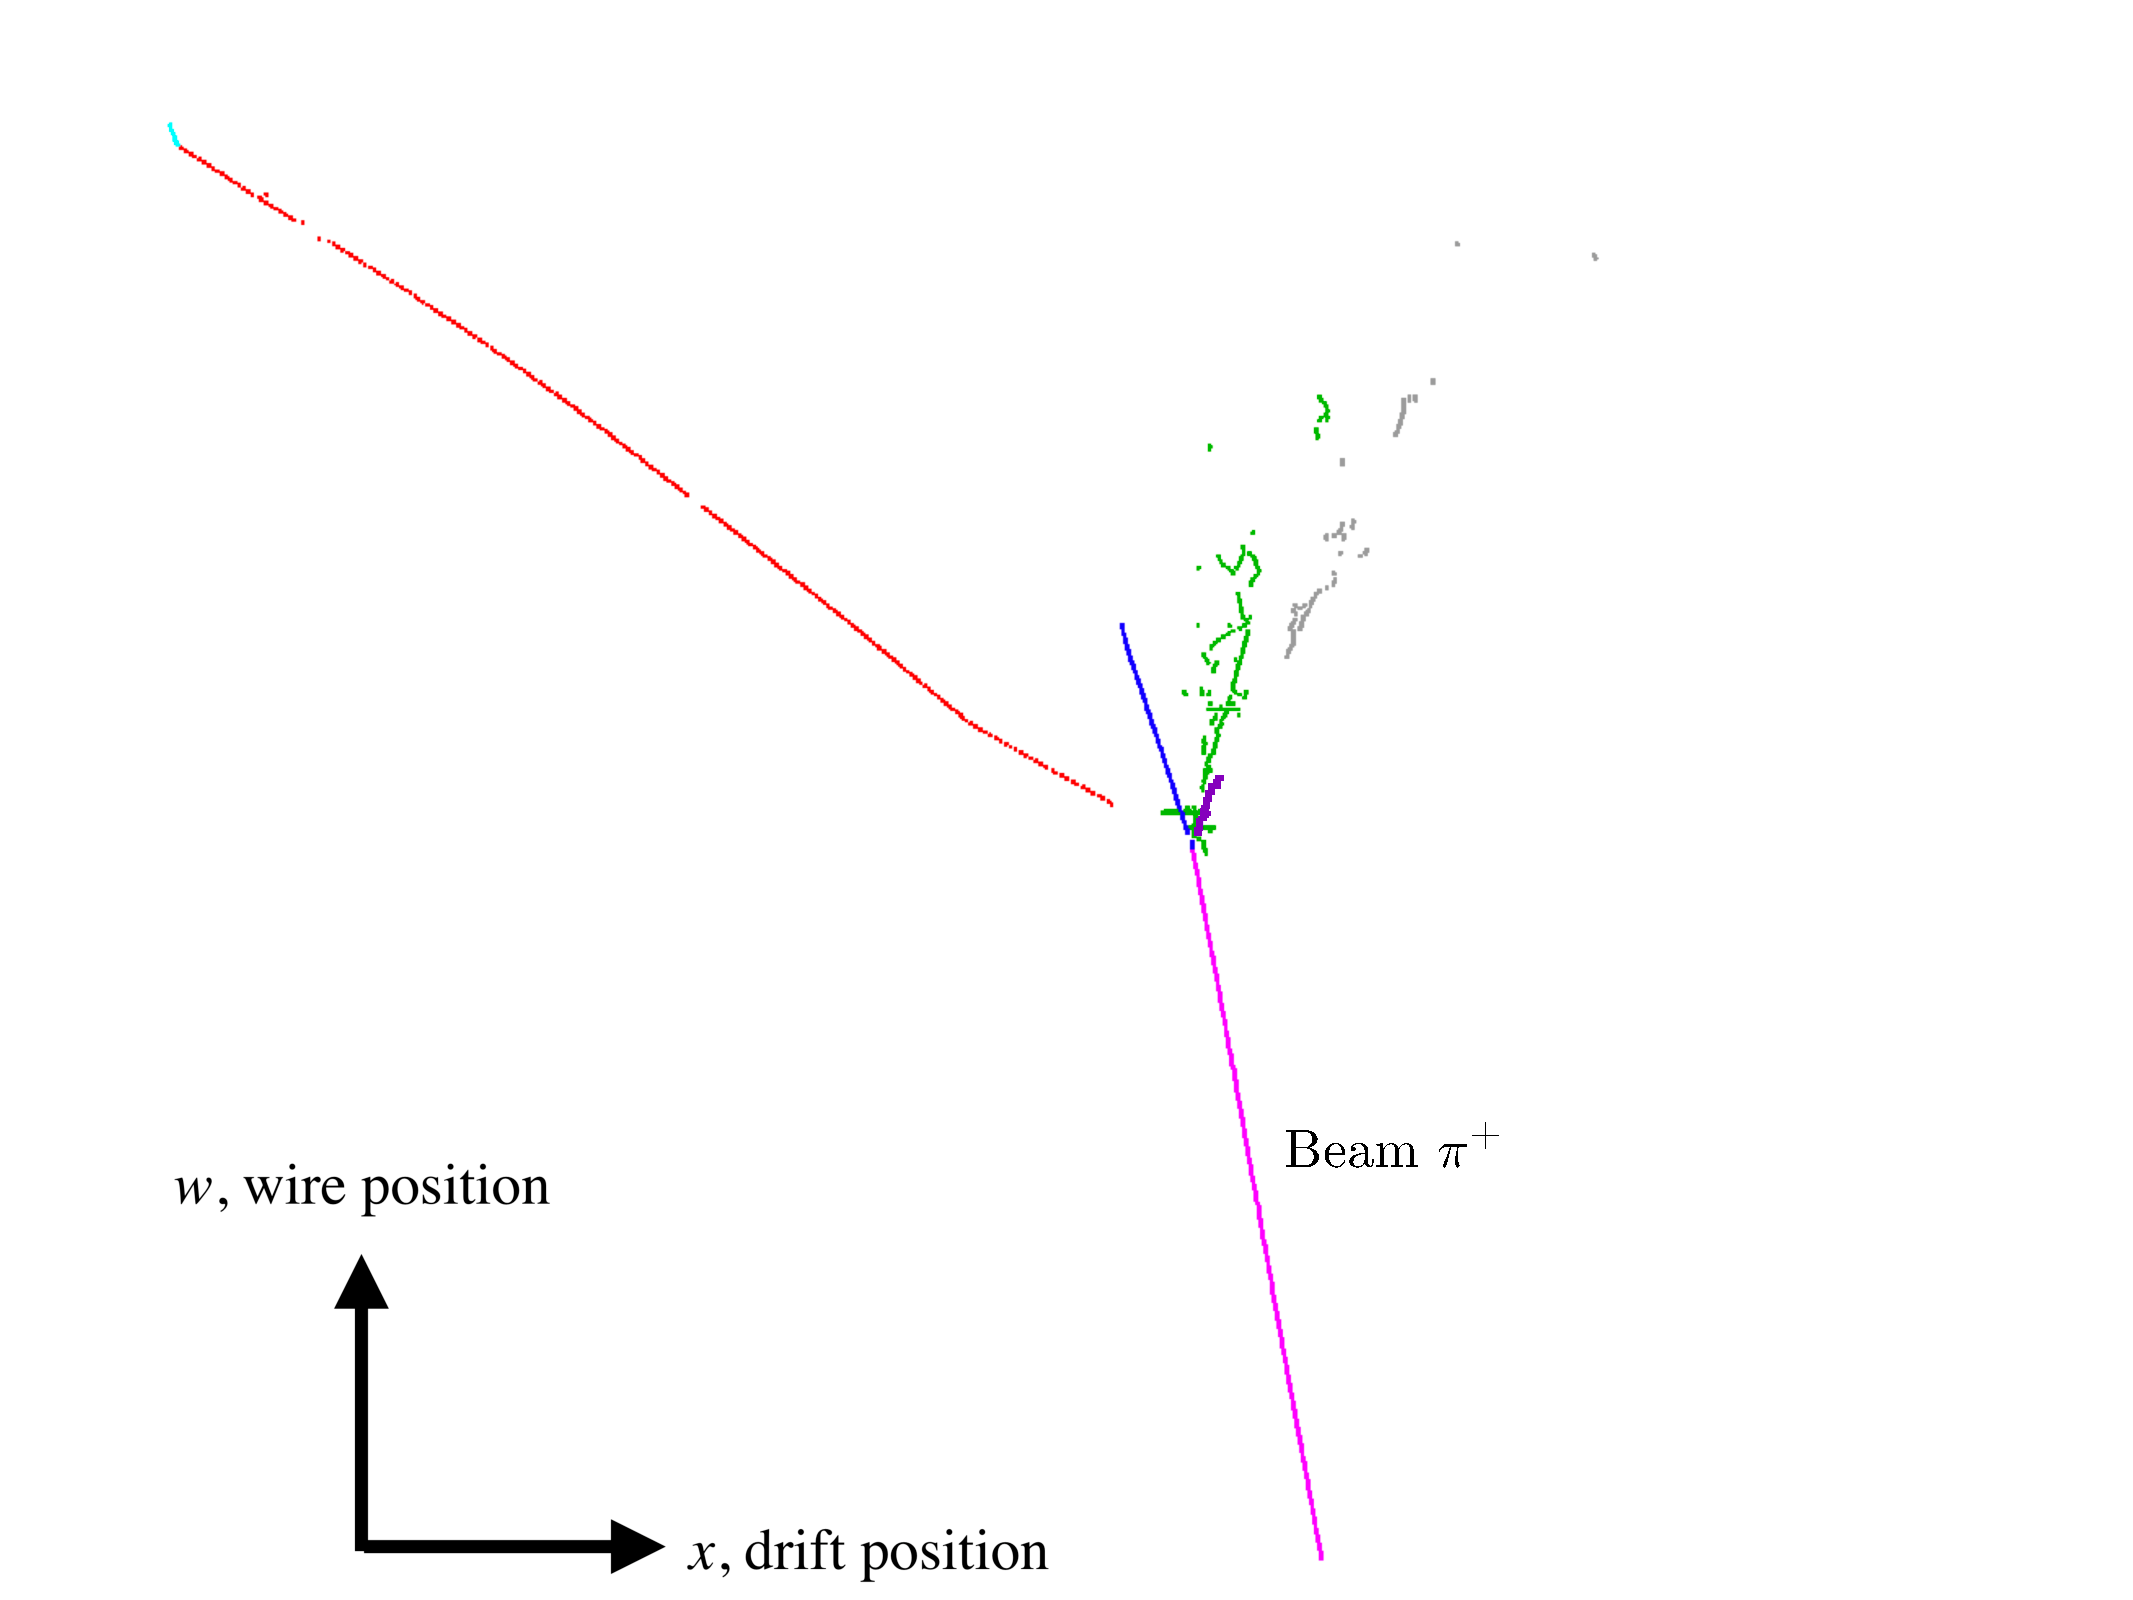
\includegraphics[width=0.9\textwidth]{figures/pandoraEvent.pdf}

	\caption
	[Reconstructed particle hierarchy from Pandora.]
	{Reconstructed particle hierarchy from Pandora. Figure from
	\cite{protoduneperf}.}

	\label{fig:pandora_pfp}

\end{figure}

As well as precise spatial reconstruction, LArTPCs provide excellent
calorimetric information. To convert the measured charge of each hit into a
reconstructed energy a number of spatial and $dQ/dx$ dependent factors need to
be taken into account. The reconstructed charge of each hit is given by the
integrated area under the gaussian fit to that hit. The $dx$ for each hit varies
based on the direction of the track with respect to the wires, it is equal to
the wire spacing divided by the sine of the angle between the wire and the 2D
projection of the track onto the anode plane.

A number of factors affect the measured $dQ/dx$, these effects need to be 
corrected in order to recover the $dQ/dx$ at the source of the ionisation. 
These factors are split into two parts in the \protodune{} reconstruction:
\begin{itemize}
	\item Corrections in the drift direction, X corrections. Examples include 
		longitudinal diffusion, attenuation on impurities, and drift velocity
		variations.
	\item Corrections in the direction of the wire planes, YZ corrections.
		Examples include wire to wire response variations, transverse diffusion, and 
		detector features such as electron diverters near the APA boundaries.
\end{itemize}
A calibration matrix is calculated for both sets of corrections by considering a
sample of cathode crossing muons. The aim of these calibration matrices is to 
normalise the response over the TPC volume based on the median of the measured
$dQ/dx$ distribution in each location. The distribution is then normalised to 
the average value at the anode plane, where the effects of the X corrections are
expected to be negligible. The corrected $dQ/dx$ is given by
\begin{equation}
	\left( dQ/dx \right)_{\mbox{corrected}} = N_Q C_{yz}(y, z) C_x(x) \left( dQ/dx
	\right)_{\mbox{reconstructed}},
\end{equation}
where $N_Q$ normalises the median of the distributions to the median value at
the anode, and $C_{yz}$ and $C_{x}$ are the calibration matrices for the YZ and 
X corrections respectively.

The final step in energy reconstruction is to convert the corrected $dQ/dx$ into
a reconstructed $dE/dx$, this involves accounting for electron--ion
recombination at the source. The modified box model is used to model the
recombination correction, this model has been studied in a LArTPC by the 
ArgoNeuT experiment \cite{Acciarri2013a}. The reconstructed $dE/dx$ is 
\begin{equation}
	\frac{dE}{dx} = \left( exp \left( \frac{\frac{dQ}{dx}}{C_{cal}} \frac{\beta^\prime
	W_{ion}}{\rho \epsilon} \right) - \alpha \right)
	\left( \frac{\rho \epsilon}{\beta^\prime} \right)
\end{equation}
where $C_{cal}$ is a calibration constant used to convert ADC to electrons,
$W_{ion}$ is the work function of argon, $\epsilon$ is the local electric field,
$\rho$ is the liquid argon density, and \(\alpha = 0.93\) and 
\(\beta\prime = 0.212 \mbox{ (kV/cm)(g/cm}^3)} / \mbox{MeV}\) are the box model 
parameters as measured by ArgoNeuT. The calibration constant, $C_{cal}$ is 
calculated by fitting the most probable value of the reconstructed $dE/dx$ 
distribution as a function of range to the theoretical prediction for $dE/dx$ 
vs range for a sample of stopping muons, as shown in figure \ref{fig:dedx_v_rr}.

\begin{figure}

	\centering

	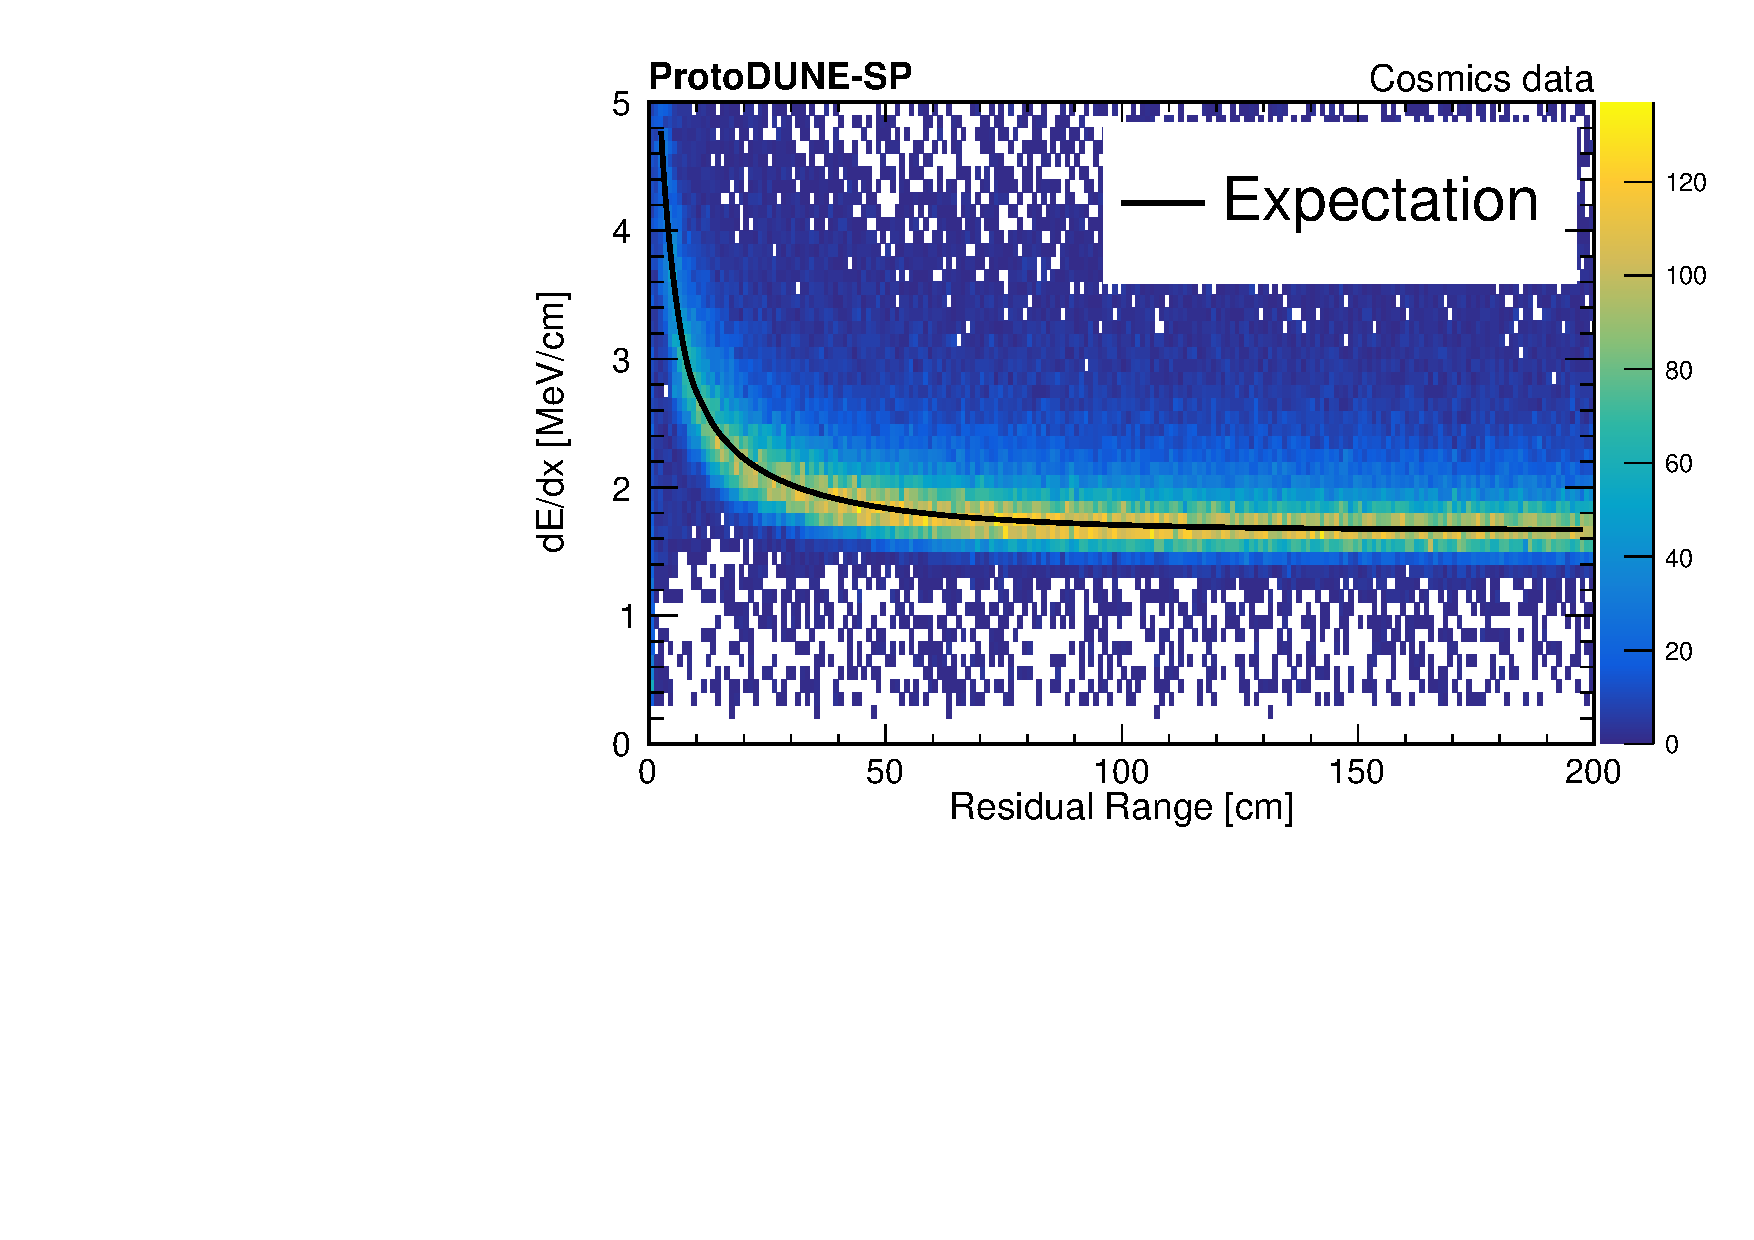
\includegraphics[width=0.9\textwidth]{figures/dedx_v_rr.pdf}

	\caption
	[$dE/dx$ vs residual range for a stopping muon sample in \protodune{} data.]
	{$dE/dx$ vs residual range for a stopping muon sample in \protodune{} data. 
	Figure from \cite{protoduneperf}.}

	\label{fig:dedx_v_rr}

\end{figure}


\section{ProtoDUNE--SP Online Monitoring System} \label{sec:pdsp_om}

As well as monitoring the stability of the detector and DAQ systems, the quality
of the collected data has to be constantly monitored. This assures the shifter 
that the data is of high quality, and prevents long runs of low quality data
being collected. The online monitoring system (OM) is responsible for 
providing this quality assurance.

As shown in Figure \ref{fig:pdsp_daq}, the OM is a part of the \protodune{} DAQ
system. The OM is responsible for processing the data and displaying
the results to the shifter in the control room as soon as possible after the
event was triggered. It consists of three main components:
\begin{itemize}
	\item Analysis processes which decode and analyse the raw data from each 
		detector subsystem.
	\item Merging processes which collate monitoring data from each subsystem.
	\item A web interface which displays monitoring data.
\end{itemize}

An overview of the data flow in the OM is shown in Figure \ref{fig:om_flow}. 
Data from the detector is first filtered before being run in any OM processes. 
The data which is passed onto the OM processes is then split up and decoded by 
the relevant RawDecoder which reformats the data ready for analysis. A number 
of Analyser modules then make use of this data to make plots, which are merged 
along with plots from external systems, and sent to a web interface to be 
displayed in the control room. The following sections will provide a brief 
summary of these stages, as well as examples of the plots which are produced 
in the OM.

\begin{figure}

	\centering

	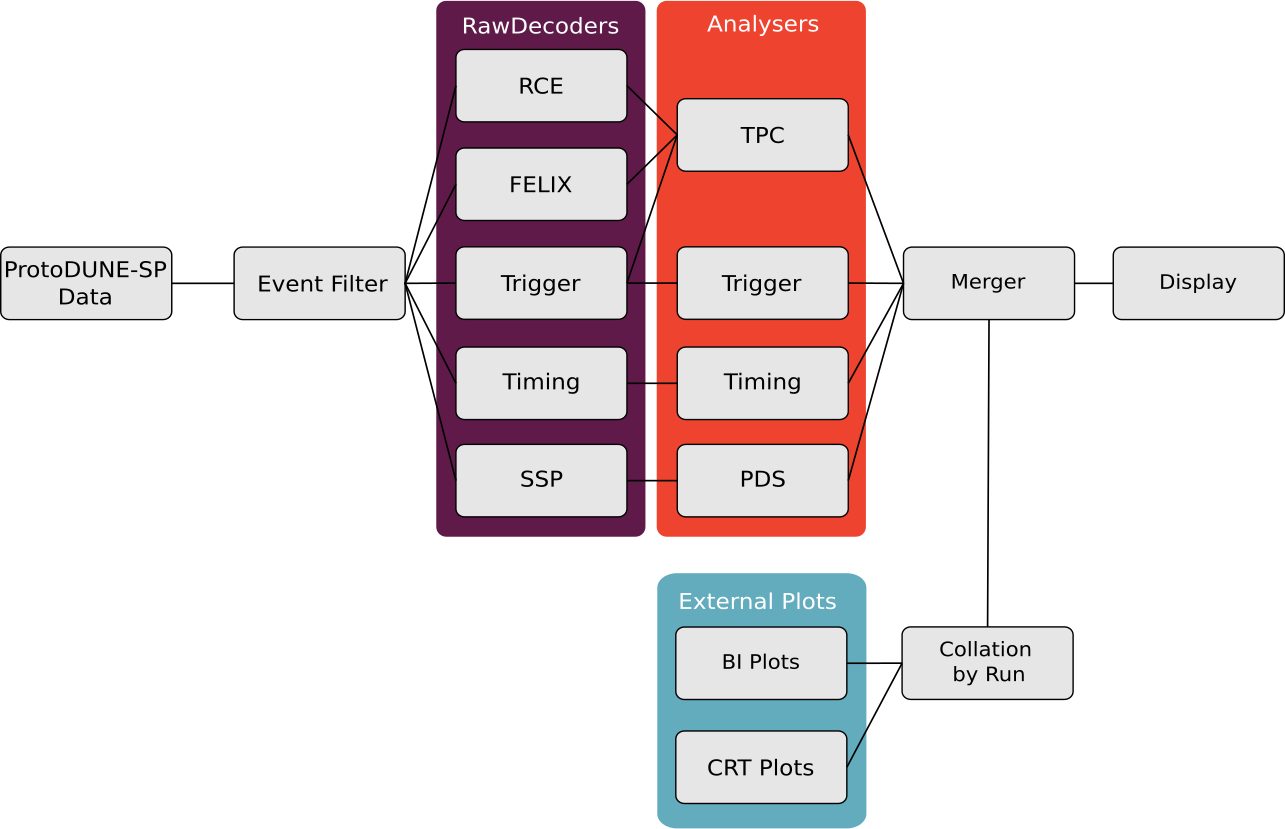
\includegraphics[width=\textwidth]{figures/om_flow.png}

	\caption
	[Data flow in the \protodune{} online monitoring system.]
	{Data flow in the \protodune{} online monitoring system.}

	\label{fig:om_flow}

\end{figure}

\subsection{Data Processing}
The data processing for the OM is based on Fermilab's art and artdaq software
frameworks \cite{Green:2012gv, 6495515}, the only exception is the beam 
instrumentation data which is analysed outside of the OM system by the CERN 
beam group. The beam instrumentation plots are merged with the rest of the OM 
plots after data processing.

The first step of the data processing is event filtering, the main purpose of
this step is to control the flow of data into the OM. Two types of filtering
take place sequentially; first a random filter is used to cut the data rate into
the OM to a manageable level, then a second filter which aims to increase the 
likelihood that processed events were triggered by the beam instrumentation or 
cosmic--ray tagger. Different OM processes take different amount of
processing time per event, therefore multiple filters are used which control the
data rate into each process separately.

After filtering the events are ready to be processed. The data coming into the
OM system is in its raw form, it arrives in small pieces known as Fragments
which have to be decoded before they can be used by the OM. The RawDecoders 
are responsible for interpreting the headers and data streams from each 
detector component, and restructuring the data ready for processing. The 
details of the decoding vary based on the readout system under consideration; 
each readout system defines a class which details the contents of each
fragment, the RawDecoders use the contents of this class to decode the fragments
to prepare the data for processing.

After the data has been decoded it is ready to be analysed, this is done by a
number of Analyser modules which analyse the data from different detector
components and produce ROOT \cite{ANTCHEVA20092499} plots as output. Details 
of the processing done for each detector component will be given below.

\subsubsection*{Time Projection Chamber}
As the largest data source in \protodune{} the TPC data was analysed in several
small steps: basic data checks, pedestals and noise, Fourier analysis, and event
displays. Examples of some of the plots produced by the TPC analysis are
detailed below.

The basic data checks are intended to quickly spot any fundamental issues with
the incoming data. An example of a basic check is to check which FEMBs are
active in the monitored events, Figure \ref{fig:active_femb} shows an example of
the number of events recorded by each FEMB on APA 1 for a sample of 10 analysed
events.

The pedestals and noise are continually evaluated by the online monitoring, this
data is displayed in the control room and used later in the monitoring chain to
flatten the background in the event displays. Basic hit removal is used to 
ensure that the pedestals and RMS are only calculated in the regions of the 
readout corresponding to noise signals. The RMS of all channels can be
represented on a single plot by arranging the channels into a 2D grid and
displaying the RMS as the colour scale on a 2D histogram, an example of this
plot is shown in Figure \ref{fig:ped_noise}.

To identify noise sources in the APA it is useful to study the Fourier transform
of the signal distribution, this allows the frequencies to be identified and the
Fourier distributions can be studied under different conditions to identify
noise sources; the cameras in the TPC where identified as a noise source in
this way. The OM therefore provides fast Fourier transforms (FFT) for each
APA, an example of the FFT for a single FEMB is shown in Figure
\ref{fig:TPC_FFT}.

\begin{figure}

	\centering

	\begin{subfigure}[b]{0.85\textwidth}
		\centering
		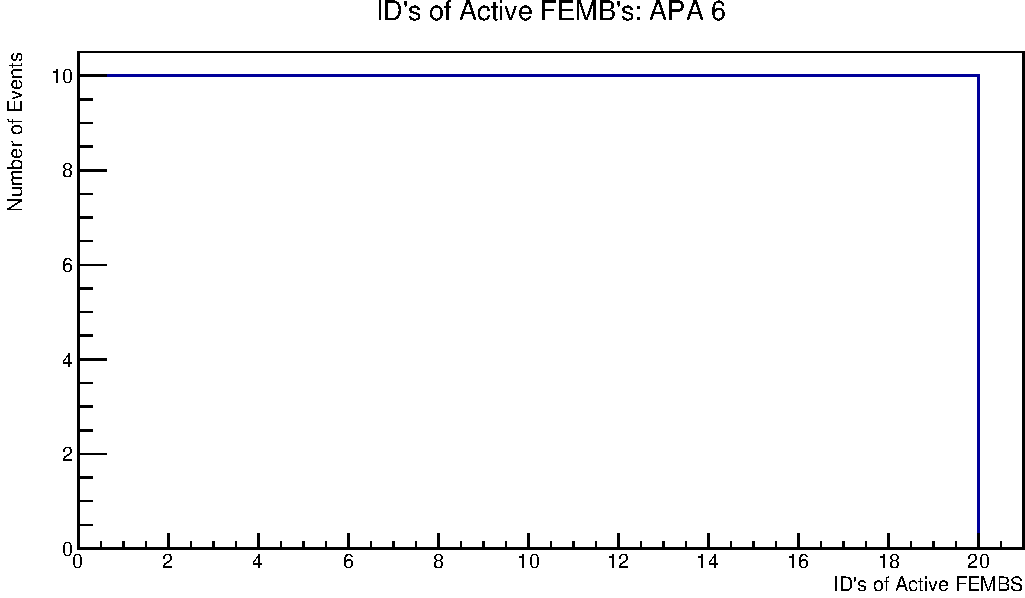
\includegraphics[width=0.9\textwidth]{figures/active_femb.pdf}
		\caption {Number of events recorded by each FEMB on APA 6.}
		\label{fig:active_femb}
	\end{subfigure}

	\begin{subfigure}[b]{0.85\textwidth}
		\raggedleft
		\vspace{3mm}
		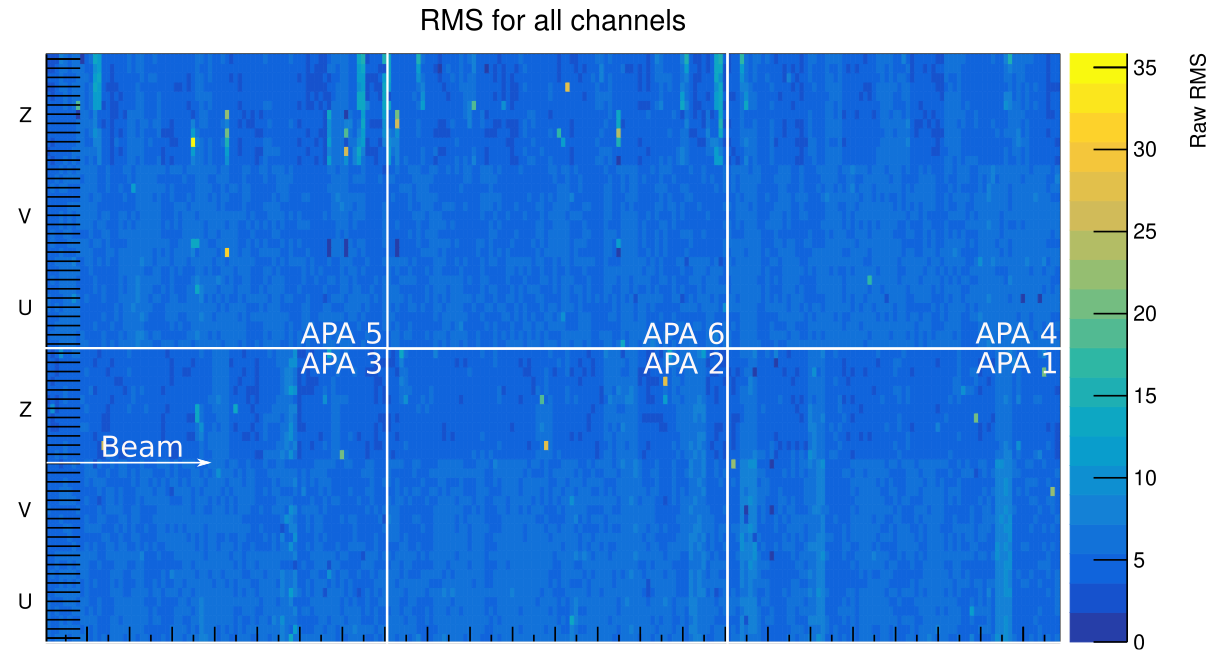
\includegraphics[width=0.95\textwidth]{figures/all_chan_rms.png}
		\caption {RMS for all channels.} 
		\label{fig:ped_noise}
	\end{subfigure}

	\begin{subfigure}[b]{0.85\textwidth}
		\centering
		\vspace{3mm}
		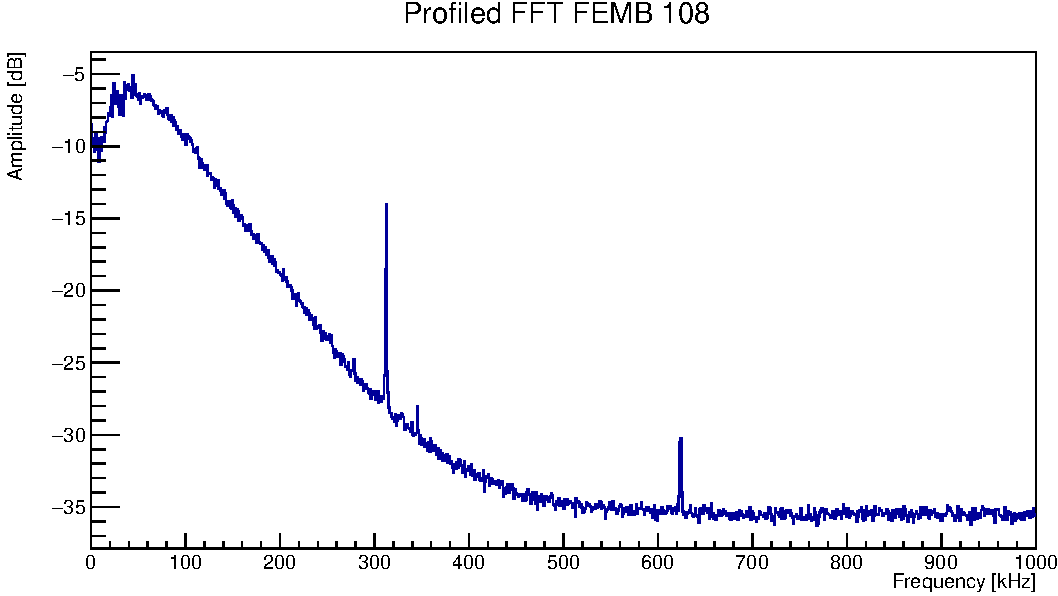
\includegraphics[width=0.9\textwidth]{figures/tpc_fft.pdf}
		\caption {FFT for a single FEMB.}
		\label{fig:TPC_FFT}
	\end{subfigure}

	\caption
	[Examples of online monitoring plots for the TPC data.]
	{Examples of online monitoring plots for the TPC data.}
	\label{fig:tpc_om}

\end{figure}

Event displays display all the data from all the TPC readout channels
simultaneously, and as such they provide the most general check of TPC 
performance in the OM. During the beam run of \protodune{} a number of issues in
the data were first identified in the event display, for example issues in the 
channel mapping and timing synchronisation. They are also particularly useful 
for checking that the beam trigger results in beam particles in the TPC. As 
a result a significant effort was made to make event displays available in 
the \protodune{} OM system; in particular changes to the display server 
were required, these will be discussed later. 

Event displays were offered for all views in all APAs, as well as a specific 
beam window event displays in each view, and stitched event displays for all 
of the APAs on each side of the TPC. As the slowest plot to make in the OM, 
only one set of event displays was made per OM output file; to maximise the 
number of beam particles in the event displays the trigger information was 
included during processing. An example of a beam window event display is shown 
in Figure \ref{fig:beam_evd}; the timing synchronisation issue mentioned
previously is visible here, this issue affects a single FEMB and is mitigated 
during offline reconstruction.  

\begin{figure}

	\centering

	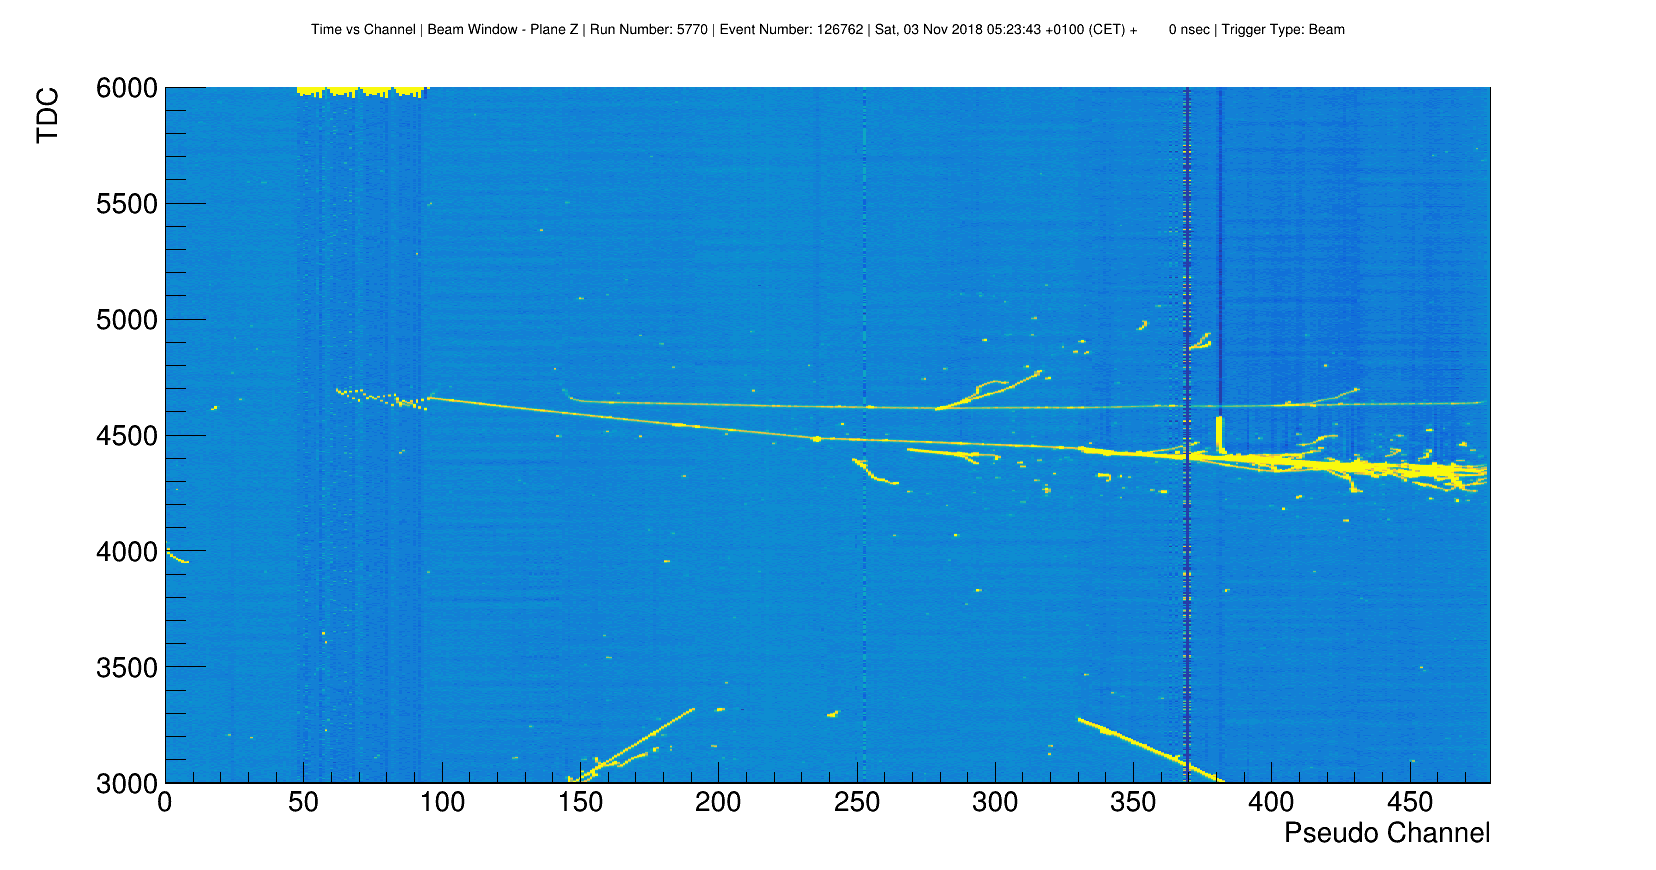
\includegraphics[width=\textwidth]{figures/beam_evd.png}

	\caption
	[An example of a beam window event display from the \protodune{} online
	monitoring system.]
	{An example of a beam window event display from the \protodune{} online
	monitoring system.}

	\label{fig:beam_evd}

\end{figure}

\subsubsection*{Photon Detection System}
Similarly to the TPC data the PDS data is analysed for pedestal, RMS, and FFTs;
in addition the raw waveforms for each channel are accumulated over a number of
events and displayed in the online monitoring. Examples of some of the PDS 
monitoring plots are shown in Figure \ref{fig:pds_om}.

\begin{figure}

	\centering

	\begin{subfigure}[b]{0.8\textwidth}
		\centering
		\vspace{3mm}
		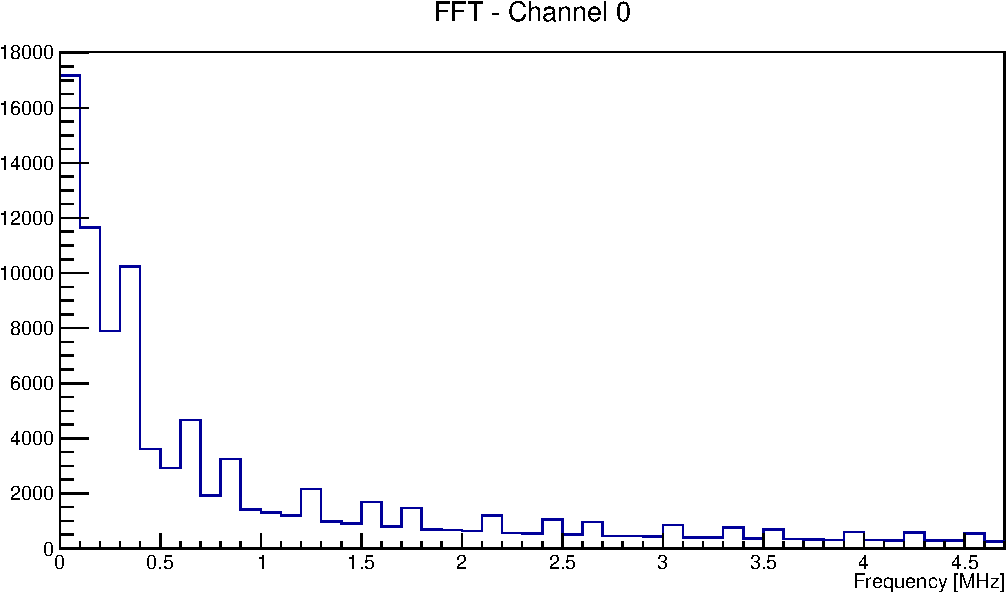
\includegraphics[width=\textwidth]{figures/pds_fft.pdf}
		\caption {FFT for a single PDS channel.}
		\label{fig:PDS_FFT}
	\end{subfigure}

	\begin{subfigure}[b]{0.8\textwidth}
		\centering
		\vspace{3mm}
		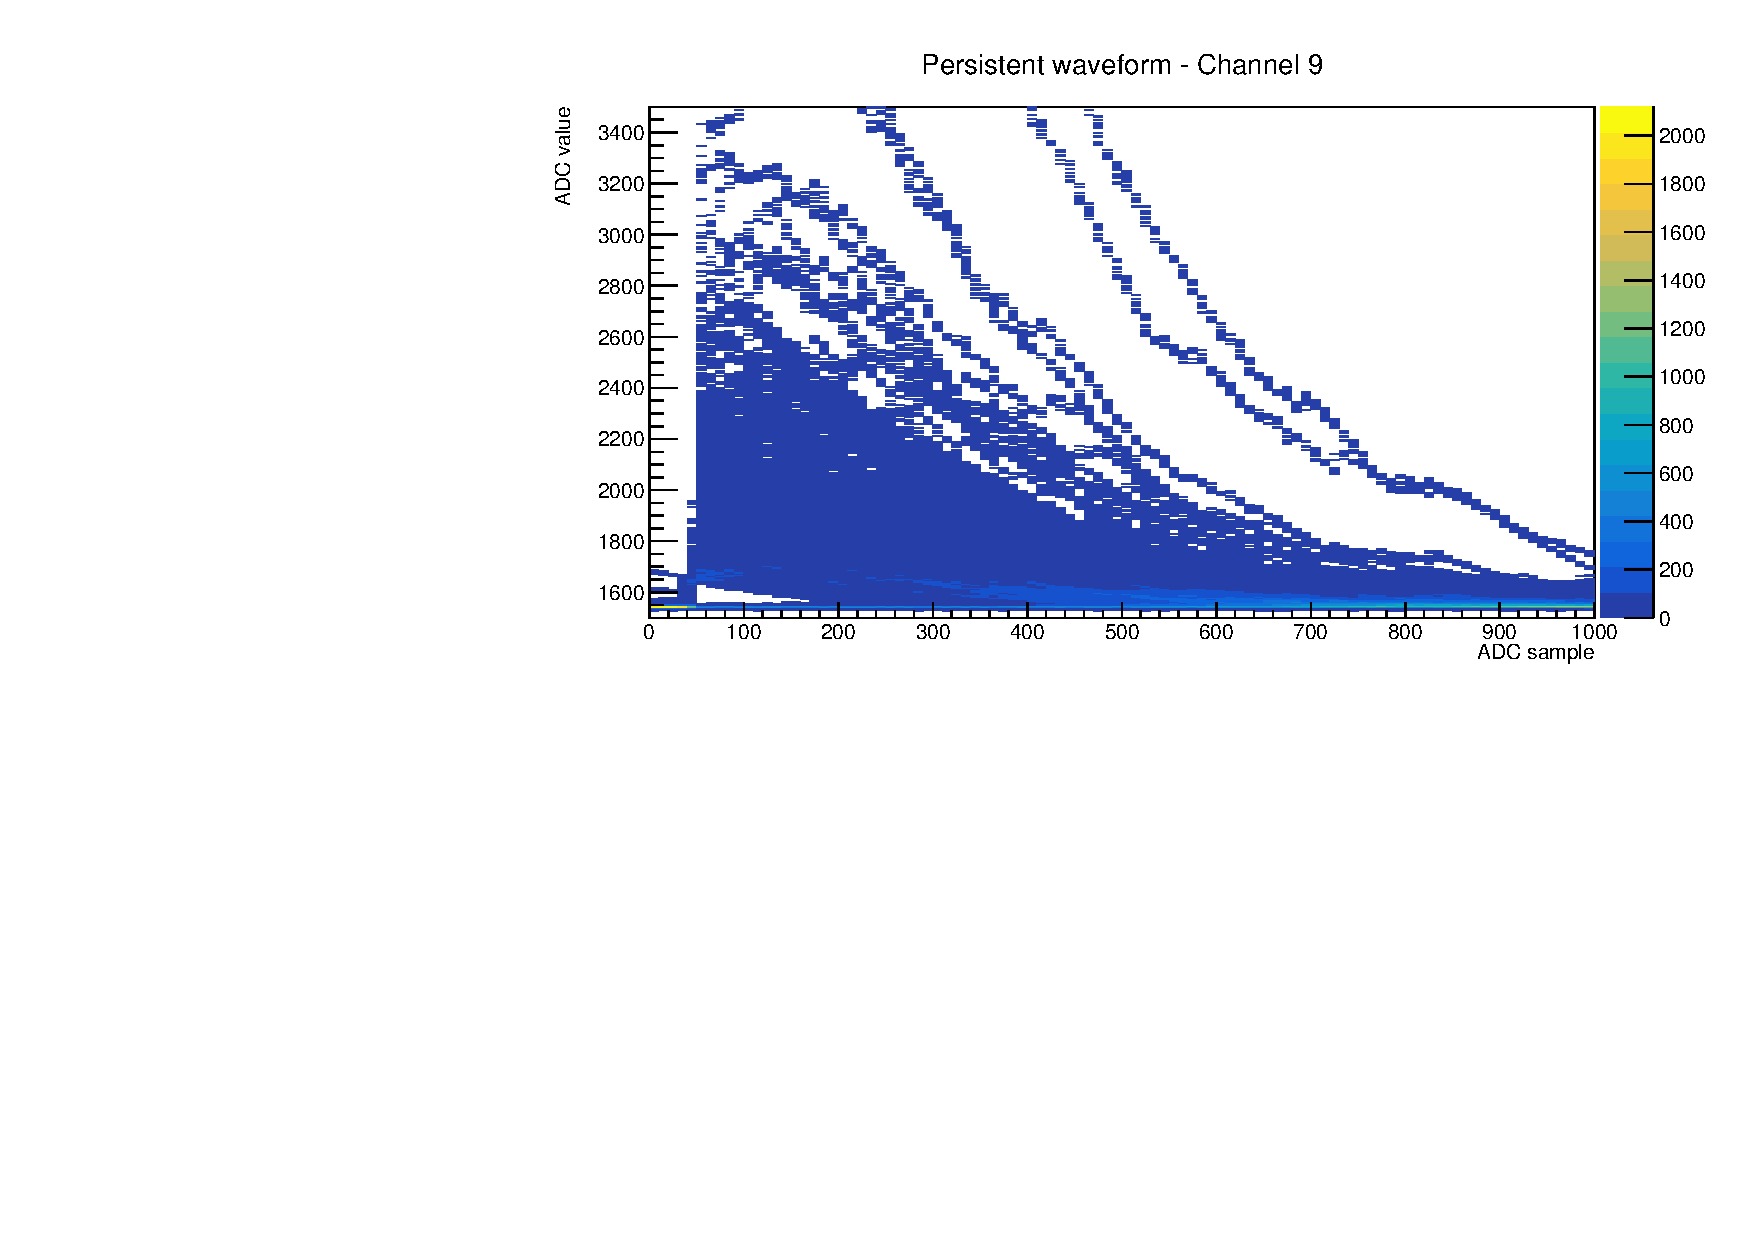
\includegraphics[width=\textwidth]{figures/pds_wav.pdf}
		\caption {Cumulative waveforms for a single PDS channel.}
		\label{fig:PDS_wav}
	\end{subfigure}

	\caption
	[Examples of online monitoring plots for the photon detection system data.]
	{Examples of online monitoring plots for the photon detection system data.}
	\label{fig:pds_om}

\end{figure}

\subsubsection*{Trigger and Timing}
The trigger and timing systems share much of the same data, because the timing
system is used to distribute the triggers from the trigger system, so their
monitoring is related. Some examples of useful timing and trigger plots include
time--stamp difference distributions, and trigger records. The time--stamp delta
plots show the difference in time--stamp between consecutive events, this
distribution can be used to monitor the stability of the trigger rate during
triggered operation. Trigger records are 2D histograms which details of
the time and type of trigger issued by the trigger board. Figure
\ref{fig:timing_OM} contains examples of these two plots.

\begin{figure}

	\centering

	\begin{subfigure}[b]{0.8\textwidth}
		\centering
		\vspace{3mm}
		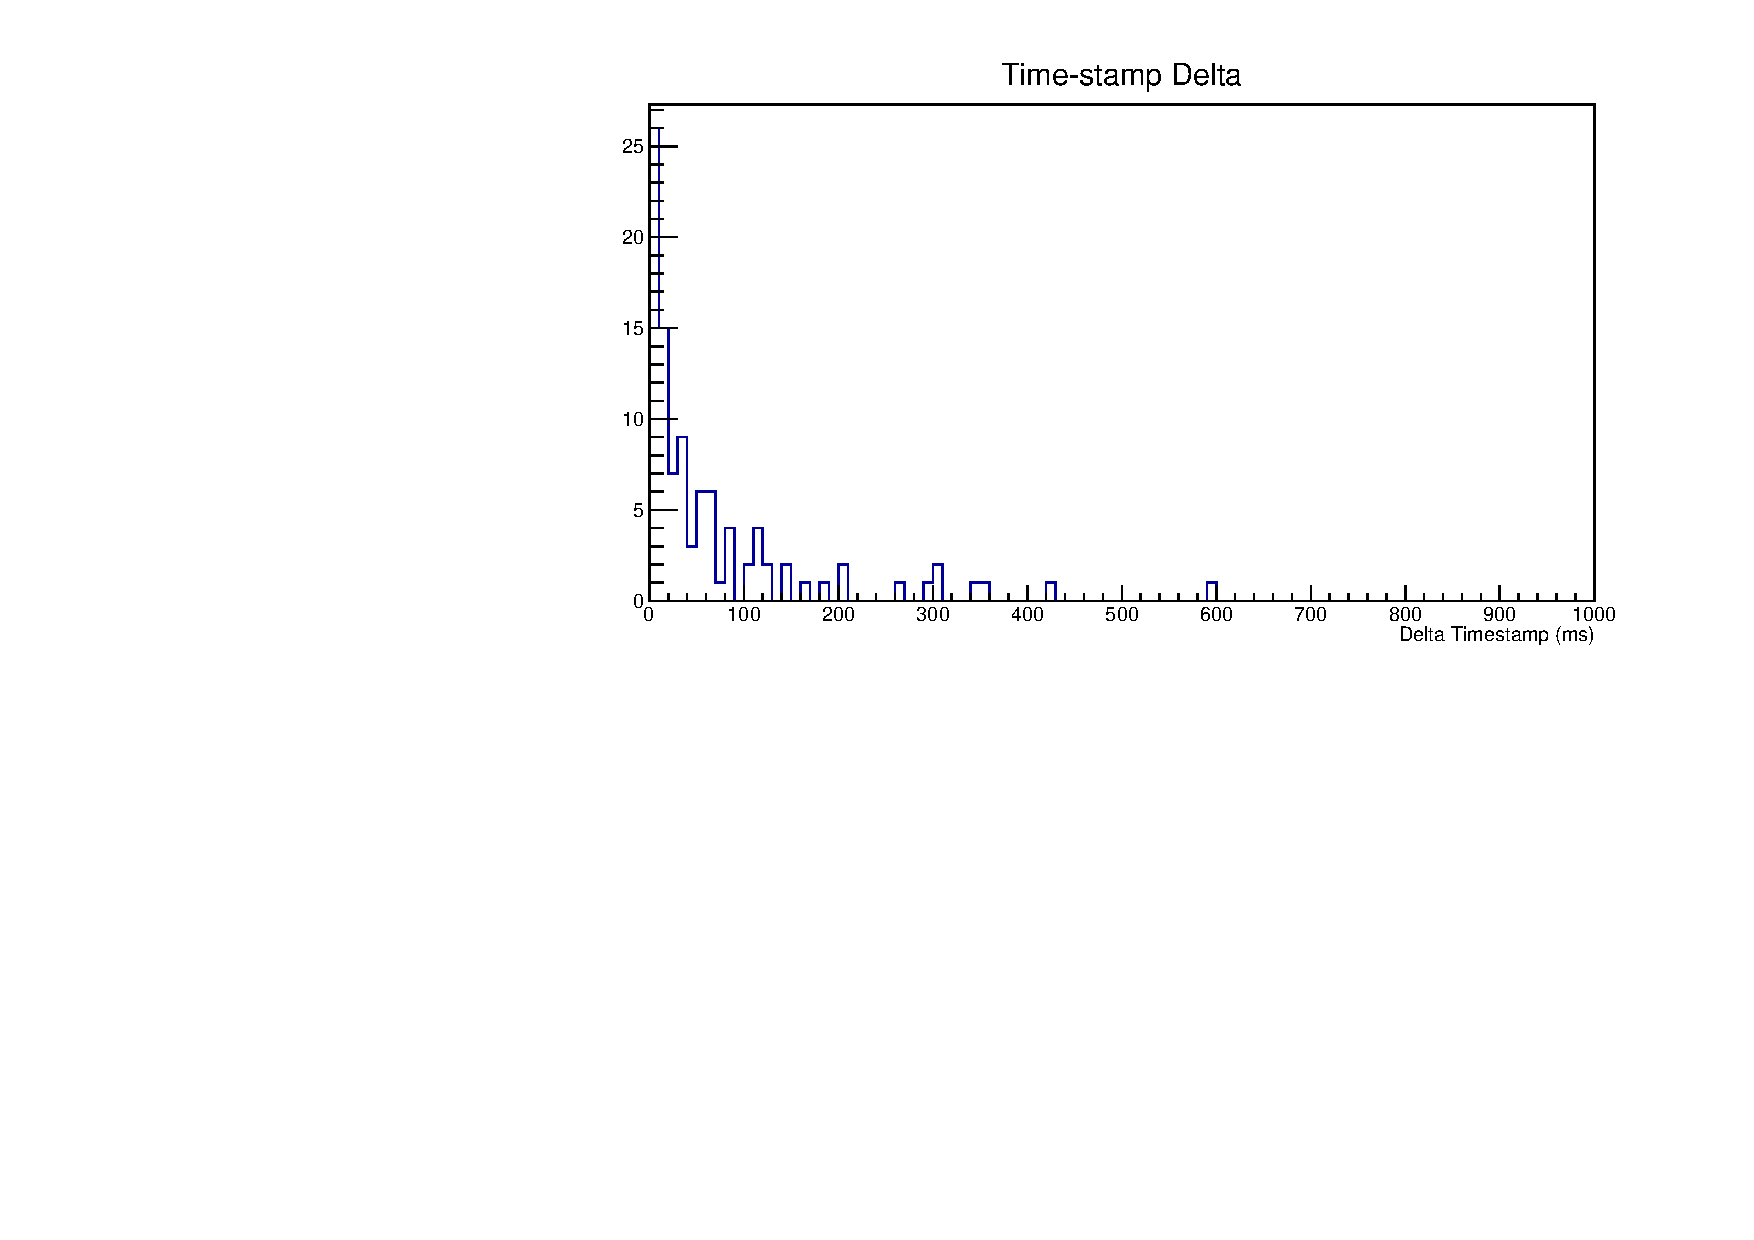
\includegraphics[width=\textwidth]{figures/timestamp_delta.pdf}
		\caption {Time--stamp delta distribution.}
		\label{fig:timestamp_delta}
	\end{subfigure}

	\begin{subfigure}[b]{0.8\textwidth}
		\centering
		\vspace{3mm}
		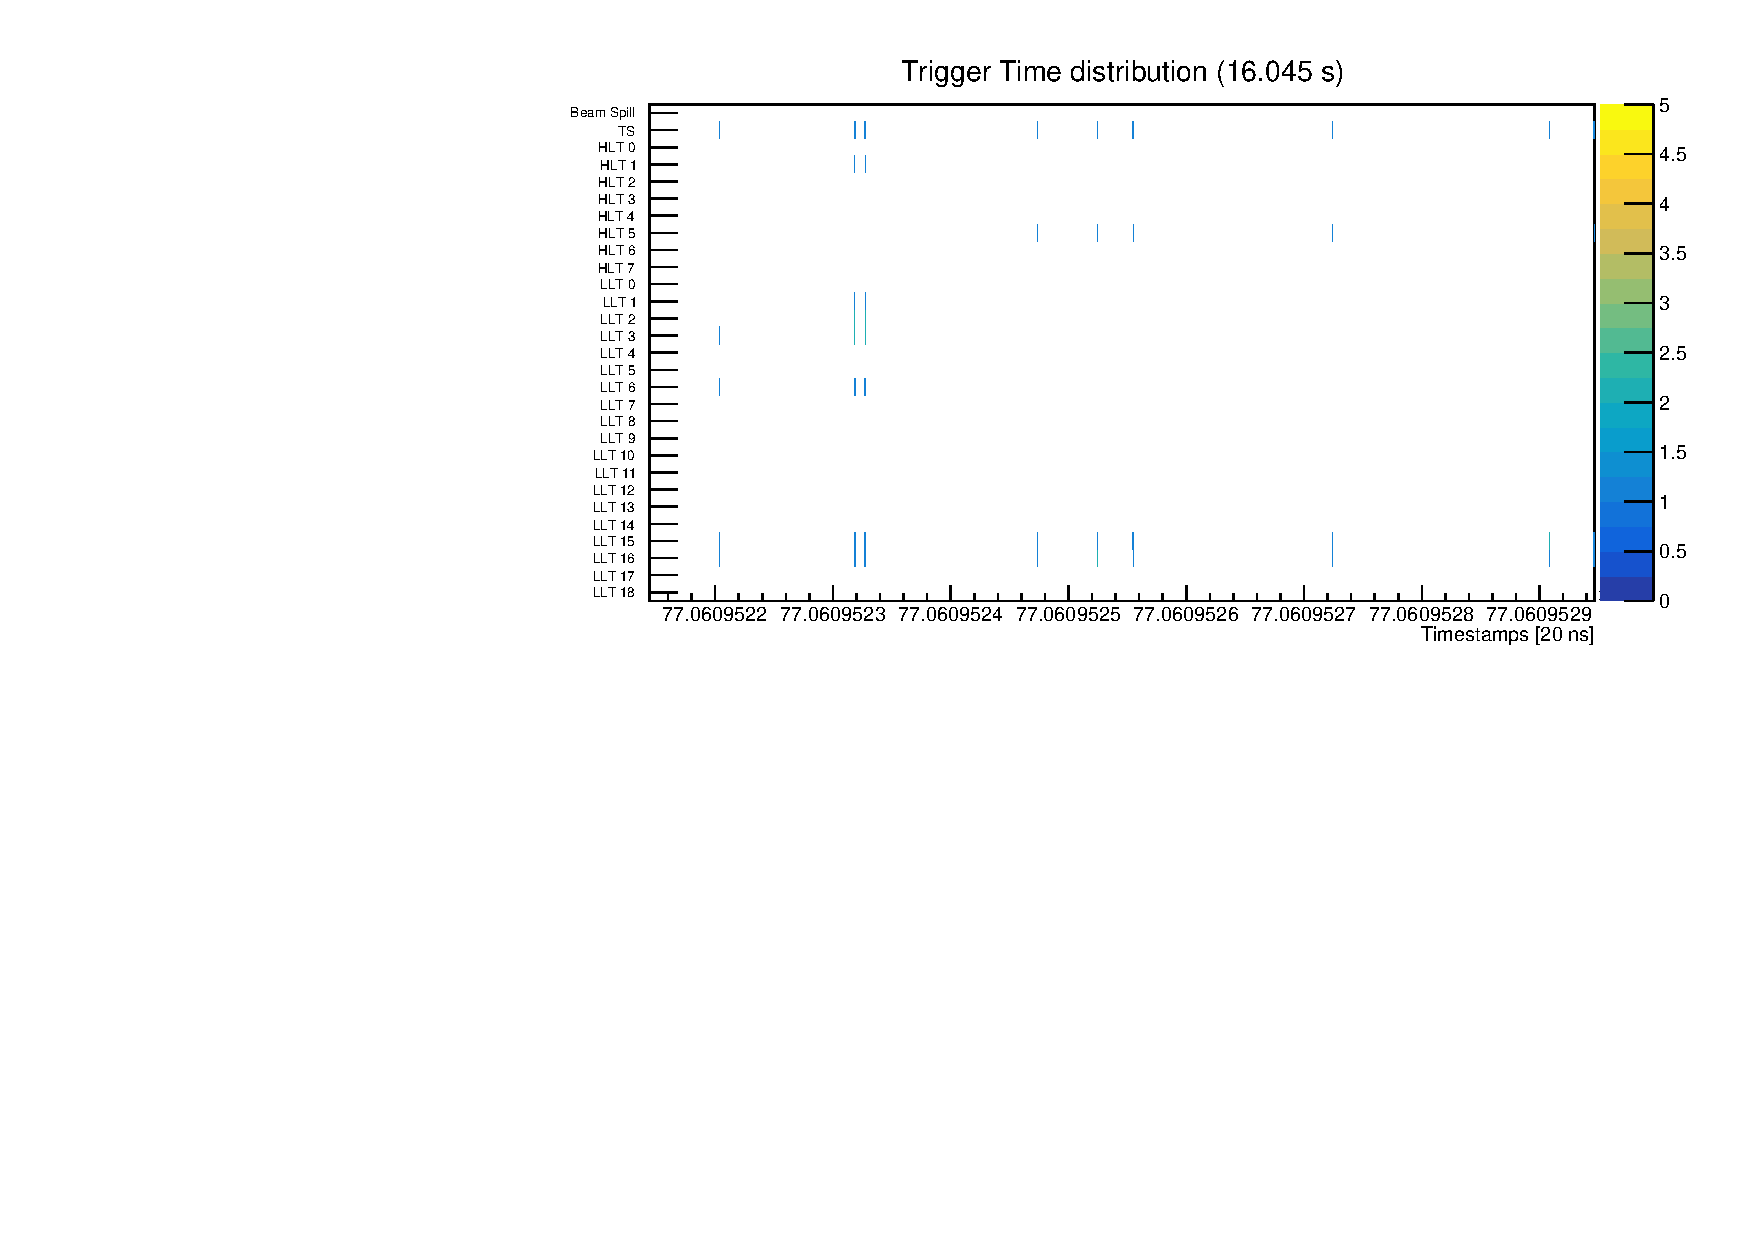
\includegraphics[width=\textwidth]{figures/trigger_record.pdf}
		\caption {Trigger records.}
		\label{fig:trig_record}
	\end{subfigure}

	\caption
	[Examples of online monitoring plots for the timing and trigger data.]
	{Examples of online monitoring plots for the timing and trigger data.}
	\label{fig:timing_OM}

\end{figure}

\subsubsection*{Beam Instrumentation}
The beamline instrumentation was monitored by CERN, who produced beamline
monitoring plots \cite{Booth:2019brj}. The plots where continually overwritten 
on a time schedule which was decoupled from the \protodune{} running schedule, 
the OM was responsible for collating the output of these plots in sync with 
the \protodune{} run schedule, such that the collated beam information for 
each run could be monitored. After collation the beam instrumentation plots 
where merged with the rest of the OM plots. The beam instrumentation plots 
included momentum, and time of flight, examples of which are shown in 
Figure \ref{fig:beam_OM}.

\begin{figure}

	\centering

	\begin{subfigure}[b]{0.8\textwidth}
		\centering
		\vspace{3mm}
		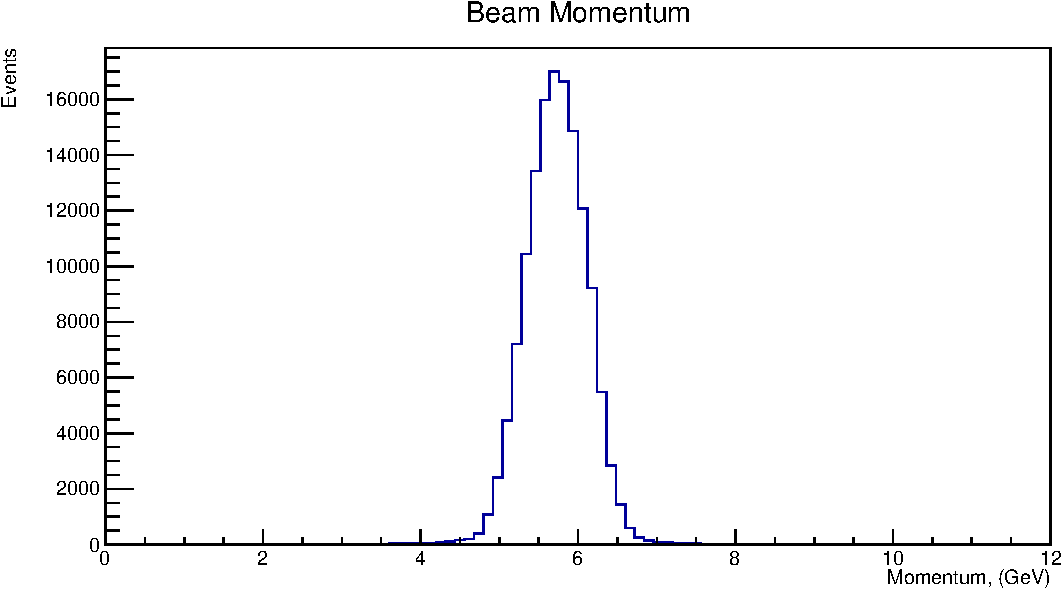
\includegraphics[width=\textwidth]{figures/beam_momentum_om.pdf}
		\caption {Beam momentum distribution.}
		\label{fig:beam_momentum_om}
	\end{subfigure}

	\begin{subfigure}[b]{0.8\textwidth}
		\centering
		\vspace{3mm}
		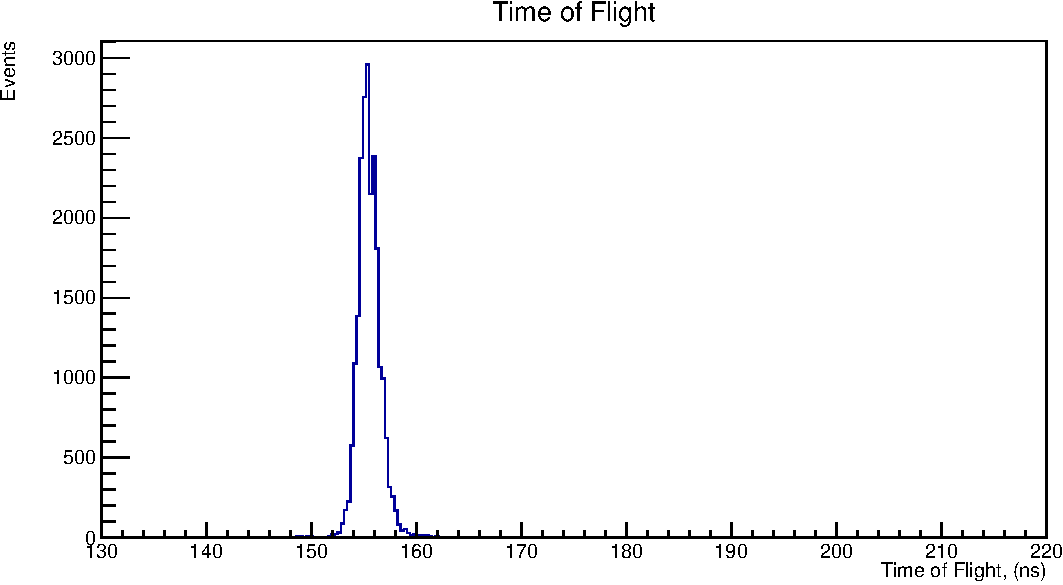
\includegraphics[width=\textwidth]{figures/beam_tof_om.pdf}
		\caption {Beam time of flight distribution.}
		\label{fig:beam_tof_om}
	\end{subfigure}

	\caption
	[Examples of online monitoring plots for the beam instrumentation.]
	{Examples of online monitoring plots for the beam instrumentation.}
	\label{fig:beam_OM}

\end{figure}

\subsubsection*{Cosmic Ray Tagger}
A bug in the DAQ meant that the CRT was run separately during the main beam 
run. Therefore, the CRT data was analysed separately from the rest of the 
\protodune{} systems and merged in the OM similarly to the beam instrumentation 
data. Some examples of CRT monitoring plots include plots of the rate of hits
for each channel, and the mean ADC for each channel, these are shown in Figure
\ref{fig:crt_OM}.

\begin{figure}

	\centering

	\begin{subfigure}[b]{0.8\textwidth}
		\centering
		\vspace{3mm}
		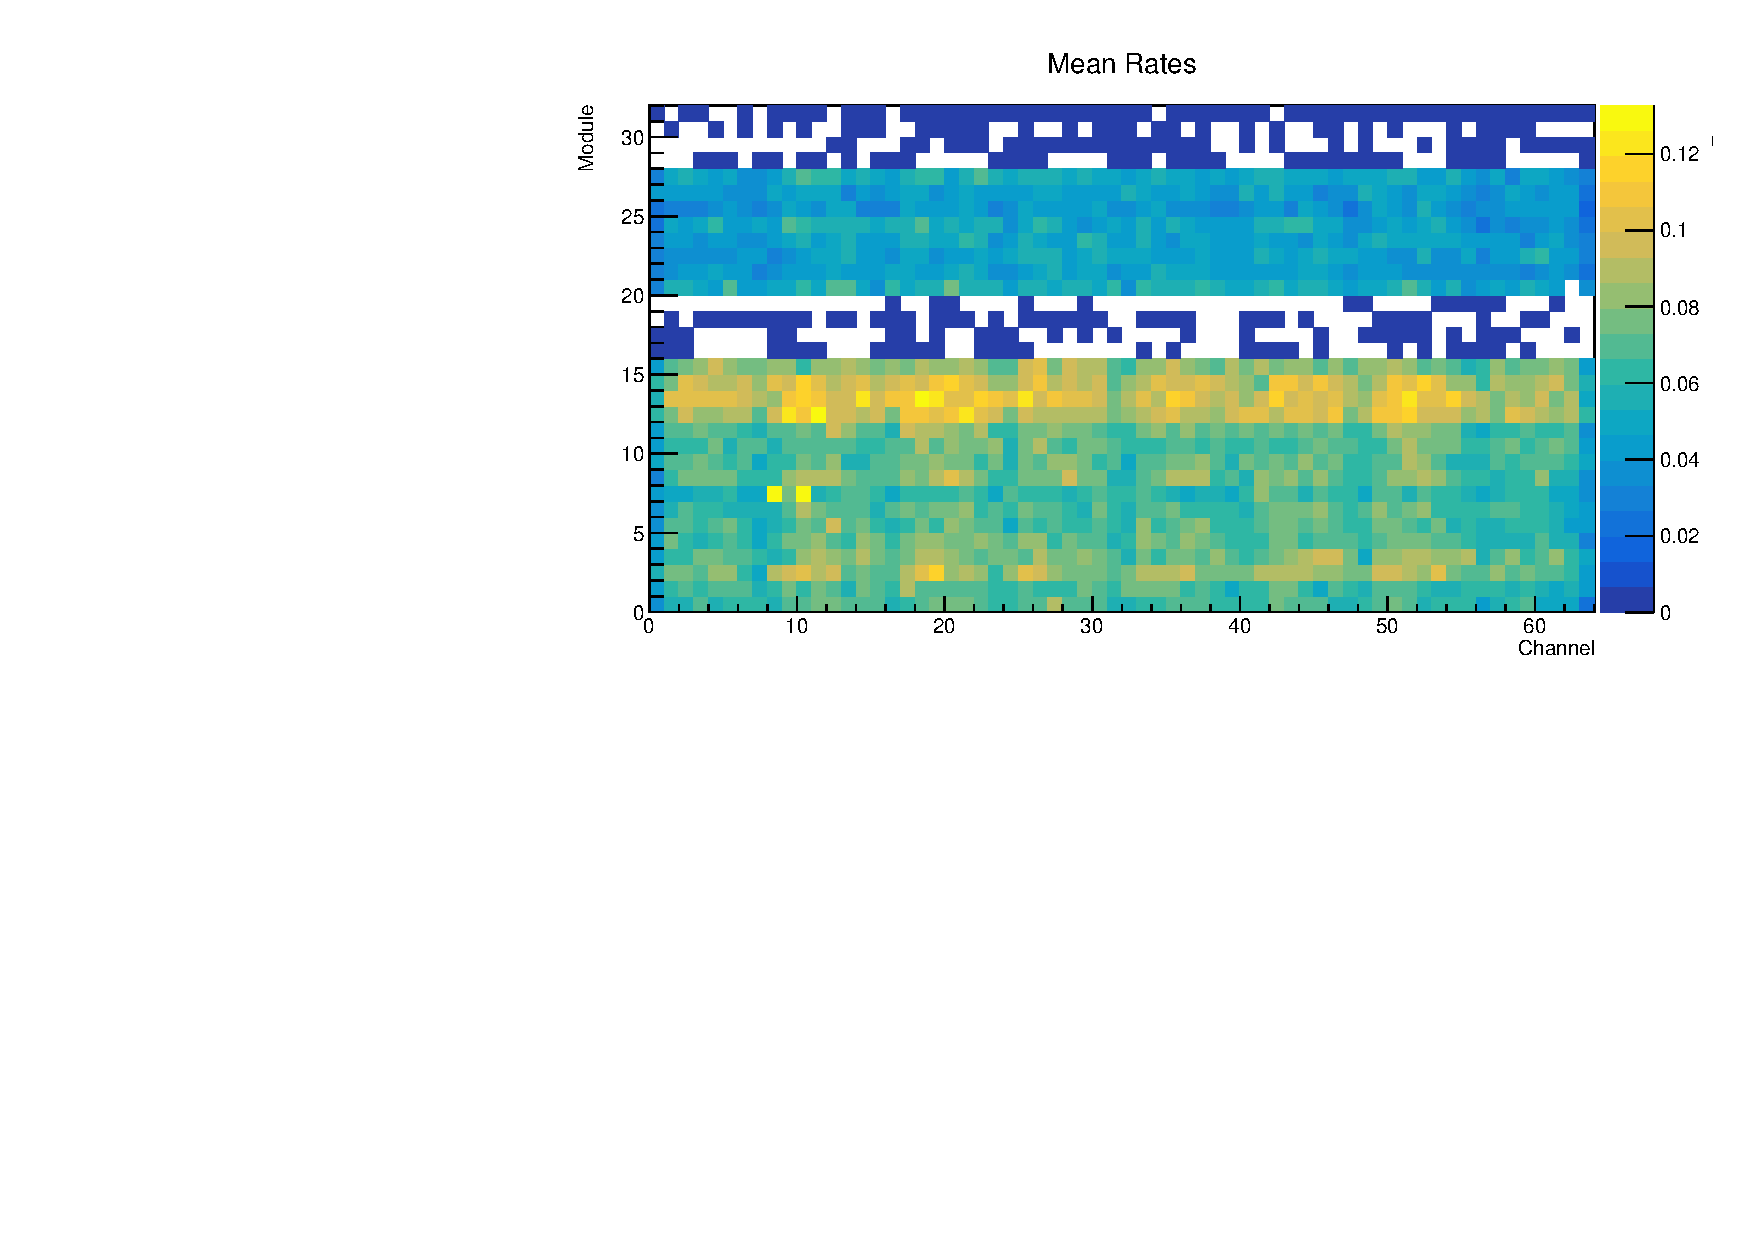
\includegraphics[width=\textwidth]{figures/crt_rate_om.pdf}
		\caption {Hit rate per channel.}
		\label{fig:crt_rate_om}
	\end{subfigure}

	\begin{subfigure}[b]{0.8\textwidth}
		\centering
		\vspace{3mm}
		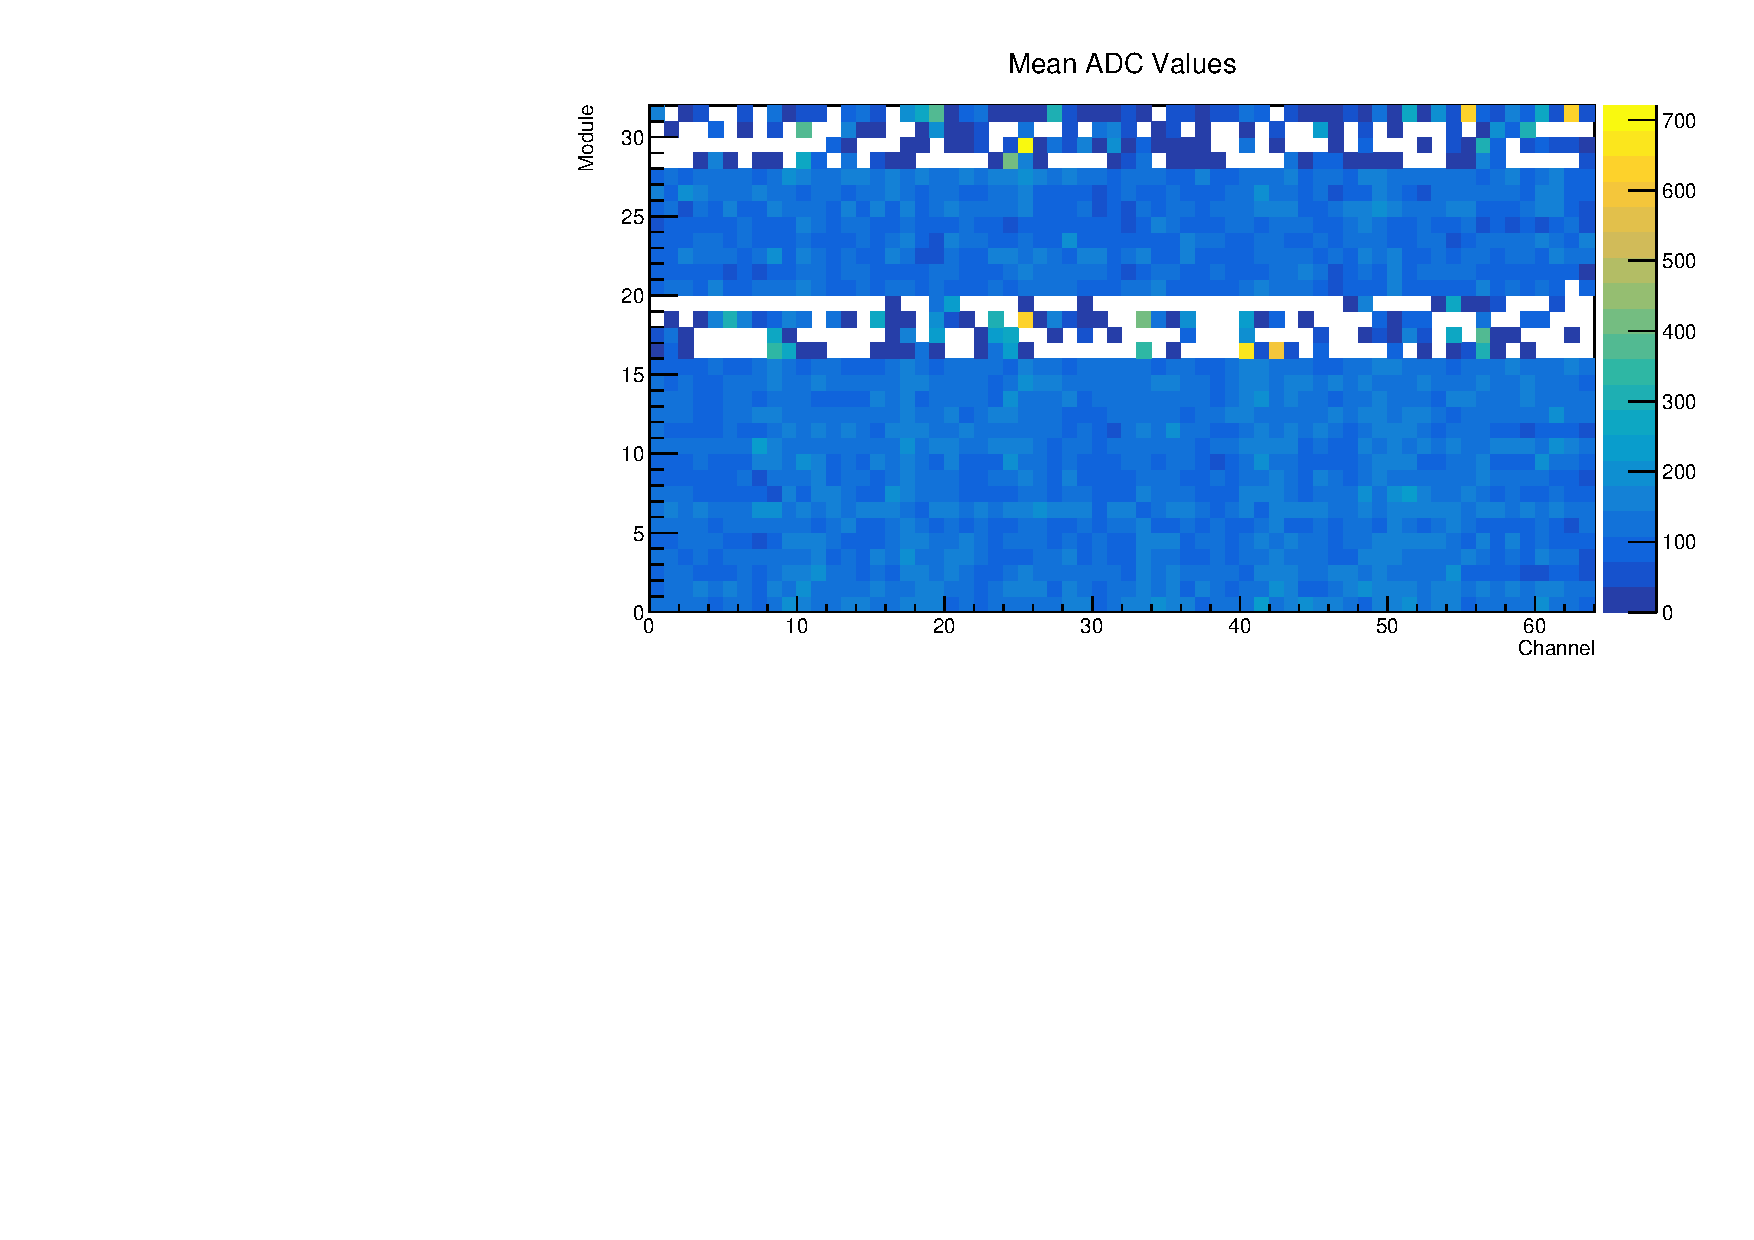
\includegraphics[width=\textwidth]{figures/crt_adc_om.pdf}
		\caption {Mean ADC per channel.}
		\label{fig:crt_adc_om}
	\end{subfigure}

	\caption
	[Examples of online monitoring plots for the cosmic ray tagger.]
	{Examples of online monitoring plots for the cosmic ray tagger.}
	\label{fig:crt_OM}

\end{figure}

\subsection{Monitoring Web Interface}
The plots from the data analysis are stored in a ROOT file on the \protodune{}
DAQ servers, this data is viewable from anywhere in CERN via a web interface
which was adapted for \protodune{} from LHCb's Monet \cite{Adinolfi_2017}. 
Monet consists of a Flask web application \cite{flask} which uses Bokeh
\cite{bokeh} to render plots for display, ROOT \cite{ANTCHEVA20092499} and 
NumPy \cite{numpy} are used to process the monitoring data in preparation for 
display.

Two important modifications were made to Monet for \protodune{}: efficiency 
improvements which were required to handle the large amounts of data in the 
event displays, and the addition of a separate rendering server with 
additional capabilities. 

The components of the web interface, and their connections, are outlined in 
Figure \ref{fig:monet_flow}. When a user makes a request, which could be a
request to open a new page of plots or a request to interact with a plot, the 
request is sent to the display server which decides what to do with it.
Depending on the nature of the request the display server will then interact
with the histogram database and/or the rendering server, before updating the
plots and displaying them to the user. 

\begin{figure}

	\centering

	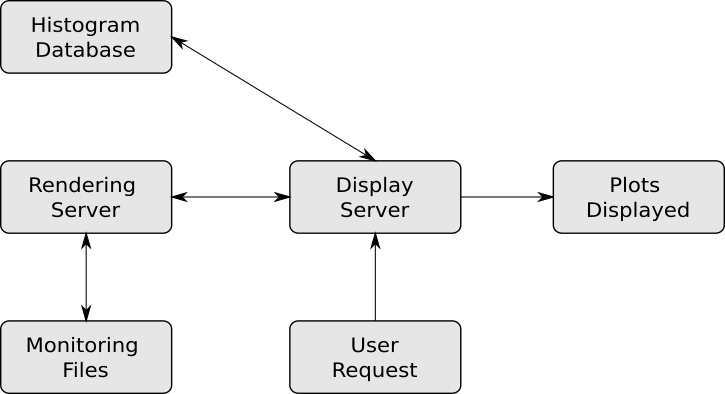
\includegraphics[width=0.7\textwidth]{figures/monet_flow.png}

	\caption
	[Data flow diagram for the web interface in the \protodune{} online 
	monitoring system.] 
	{ Data flow diagram for the web interface in the \protodune{} online 
	monitoring system. } 
	\label{fig:monet_flow}

\end{figure}

The plots in the monitoring files are organised into pages in Monet. Each page
can contain any number of plots which are organised into an array on the screen,
an example of this is shown in Figure \ref{fig:monet_page}. The histogram 
database is responsible for the details of each of these pages, this includes
the plots on each page, their locations, and the relevant rendering options for
each plot. When a new page is requested the display server requests these
details from the histogram database before requesting the rendering server to 
render the plots.

\begin{figure}

	\centering

	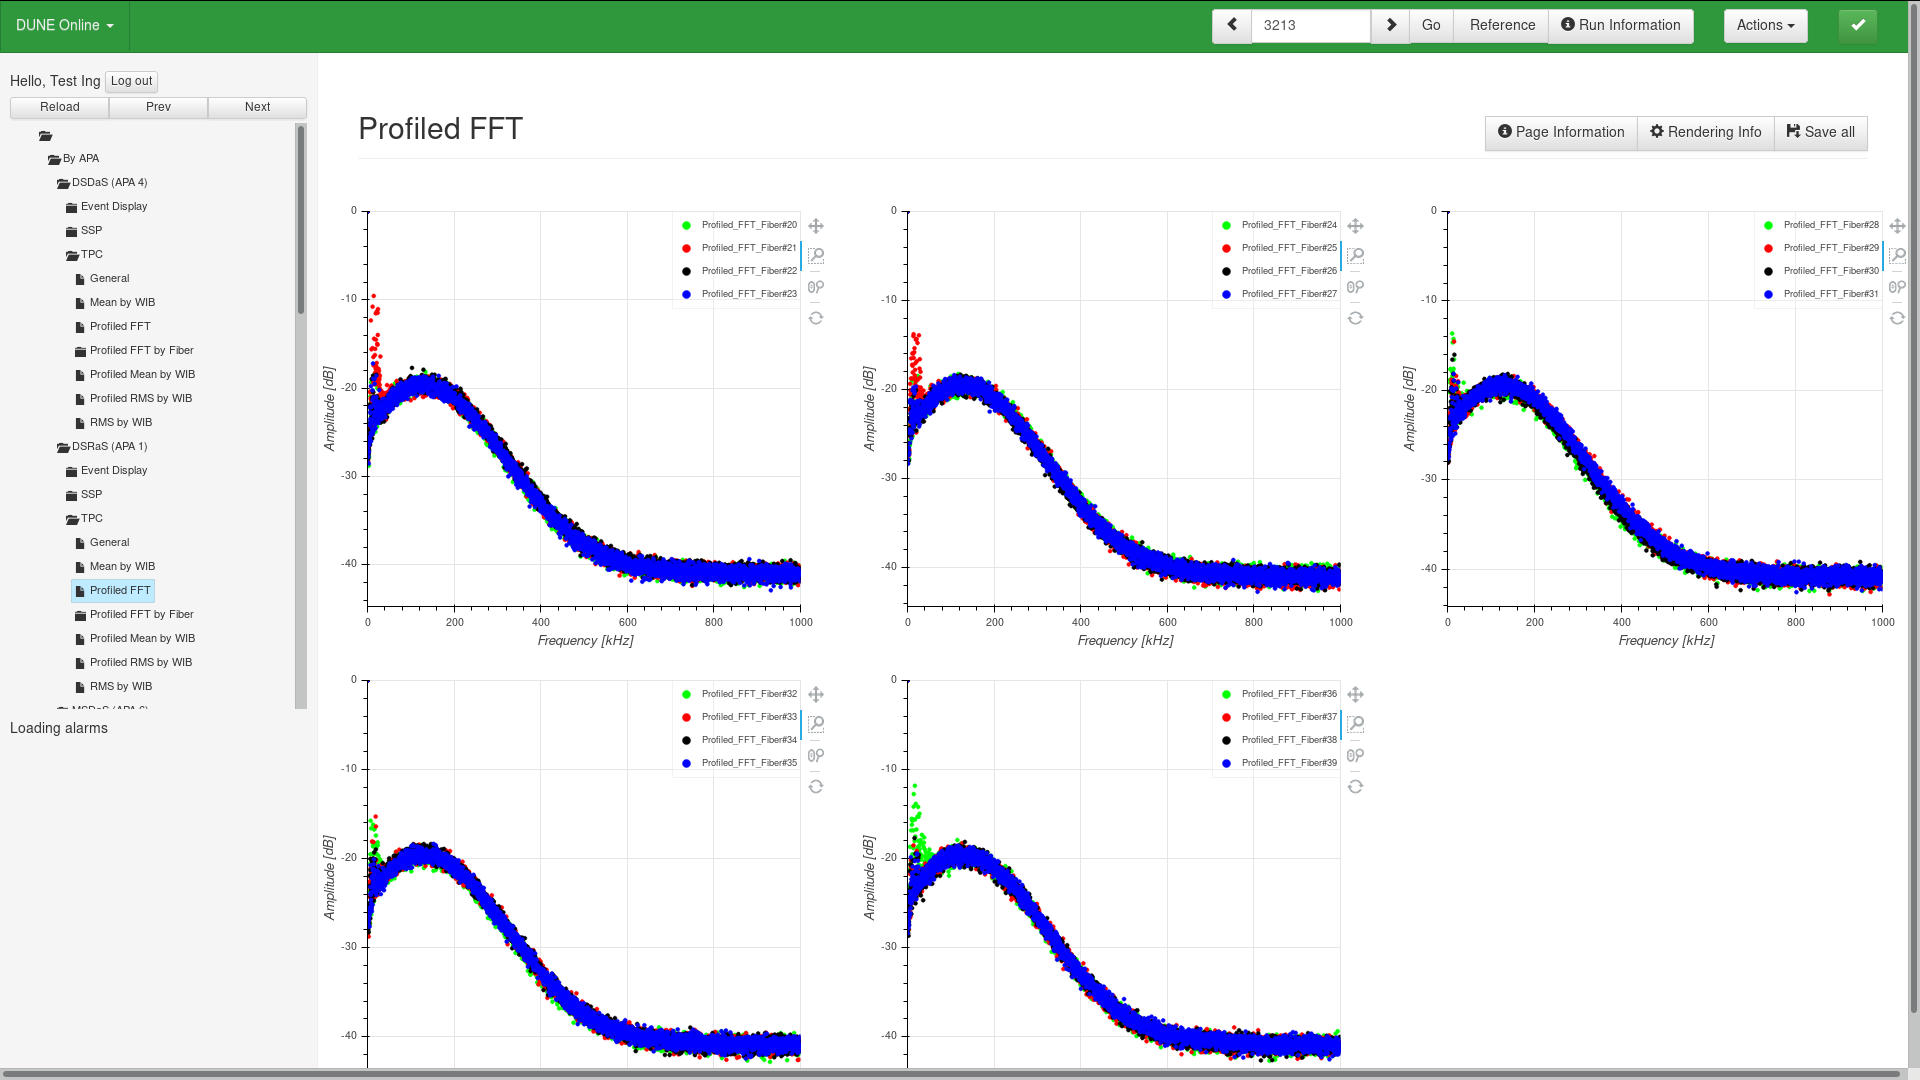
\includegraphics[width=\textwidth]{figures/profiled_fft_monet.png}

	\caption
	[An example of an online monitoring page.] 
	{ An example of an online monitoring page, profiled FFTs for APA 1. } 
	\label{fig:monet_page}

\end{figure}

The rendering server is responsible for rendering the plots from the monitoring
ROOT files, it is capable of rendering all 1D and 2D ROOT plots. In LHCb's Monet
rendering is handled directly on the display server, however in \protodune{} an
additional rendering server was added. By separating the rendering processes 
onto their own server additional functionality was possible. The main 
advantage of the rendering server was that it enabled the OM to utilise a 
dynamic binning algorithm to scale the resolution of the displayed images in 
response to user interaction. This is mainly used for the event displays; the 
event display is initially loaded in a low resolution, but if a user is 
interested in a specific region of the event display then they can zoom in on 
the region of interest, which is then displayed at a higher resolution by the 
dynamic binning algorithm, as demonstrated in Figure \ref{fig:dynamic_binning}.

\begin{figure}

	\centering

	\begin{subfigure}[b]{\textwidth}
		\centering
		\vspace{3mm}
		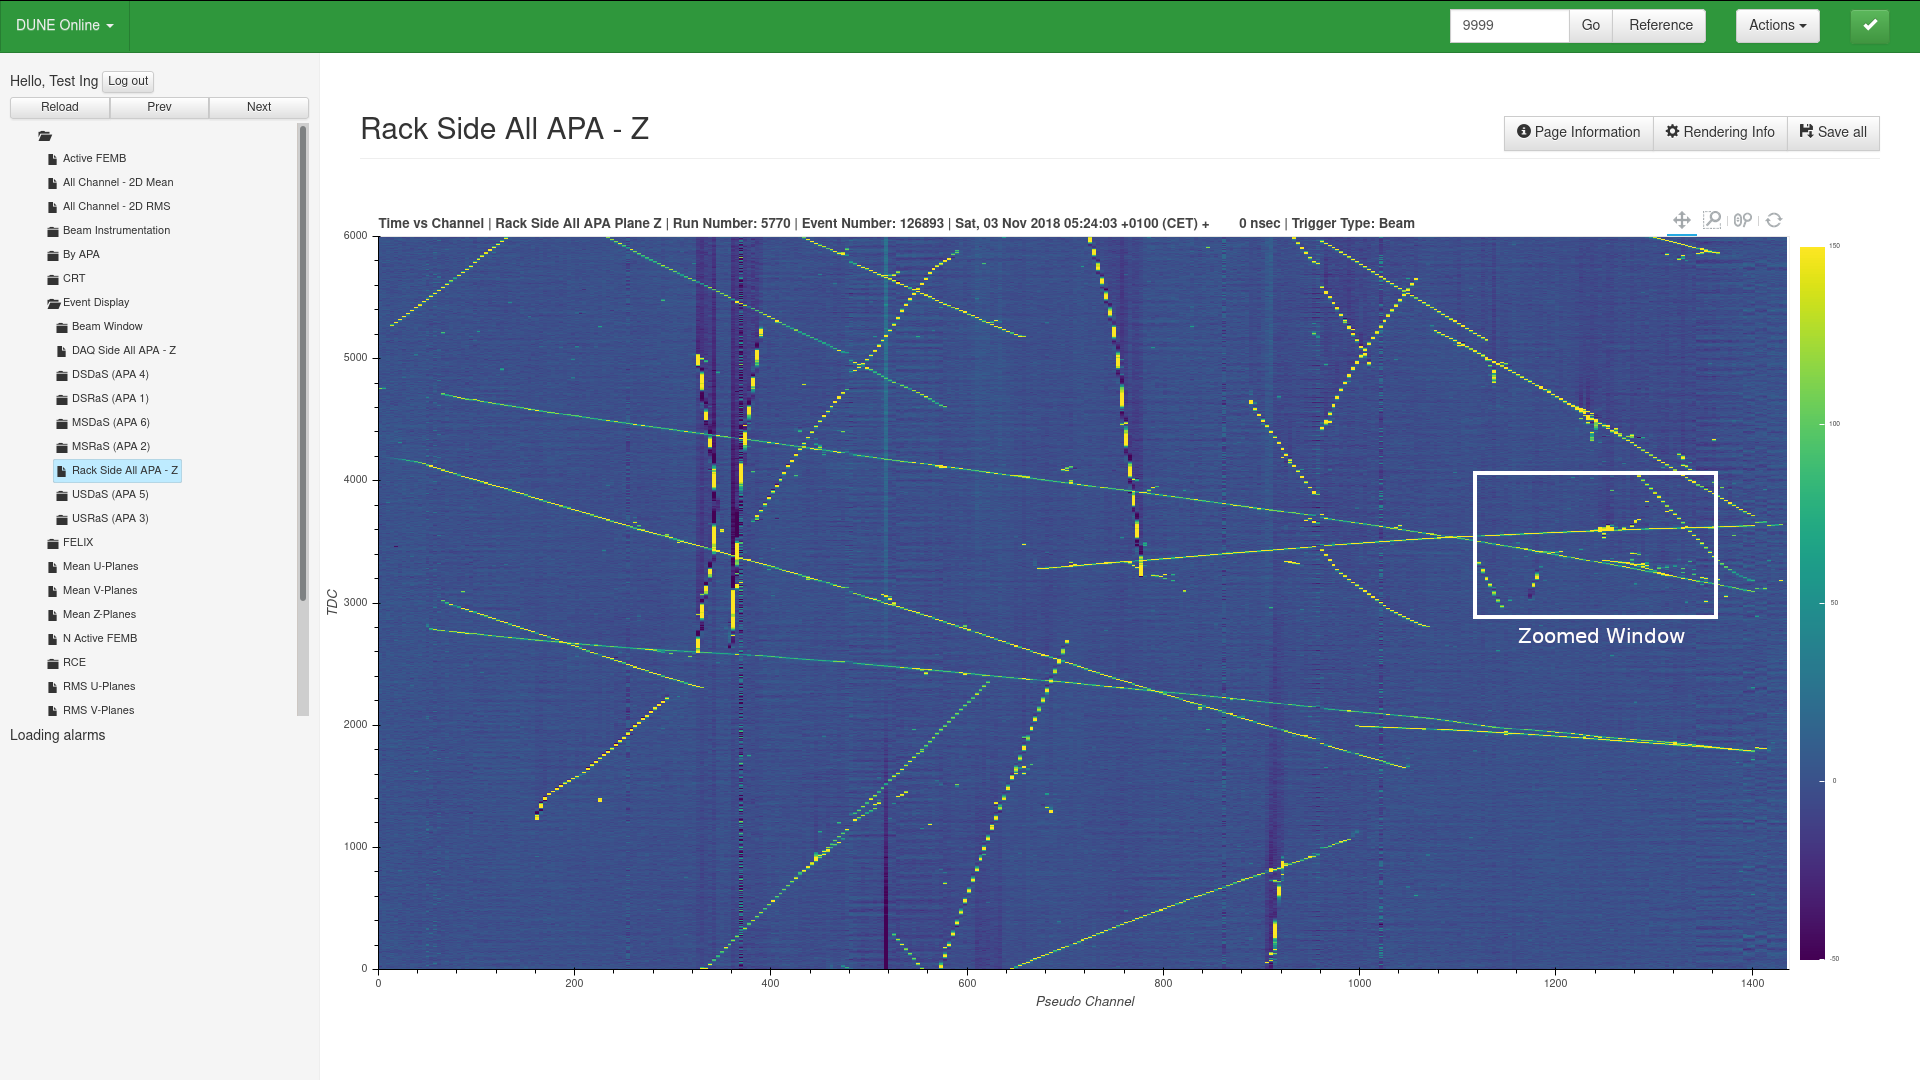
\includegraphics[width=\textwidth]{figures/zoomed_out.png}
		\caption {Full APA view. The white square represents the zoomed region in
		Figure \ref{fig:zoomed_in}.}
		\label{fig:zoomed_out}
	\end{subfigure}

	\begin{subfigure}[b]{\textwidth}
		\centering
		\vspace{3mm}
		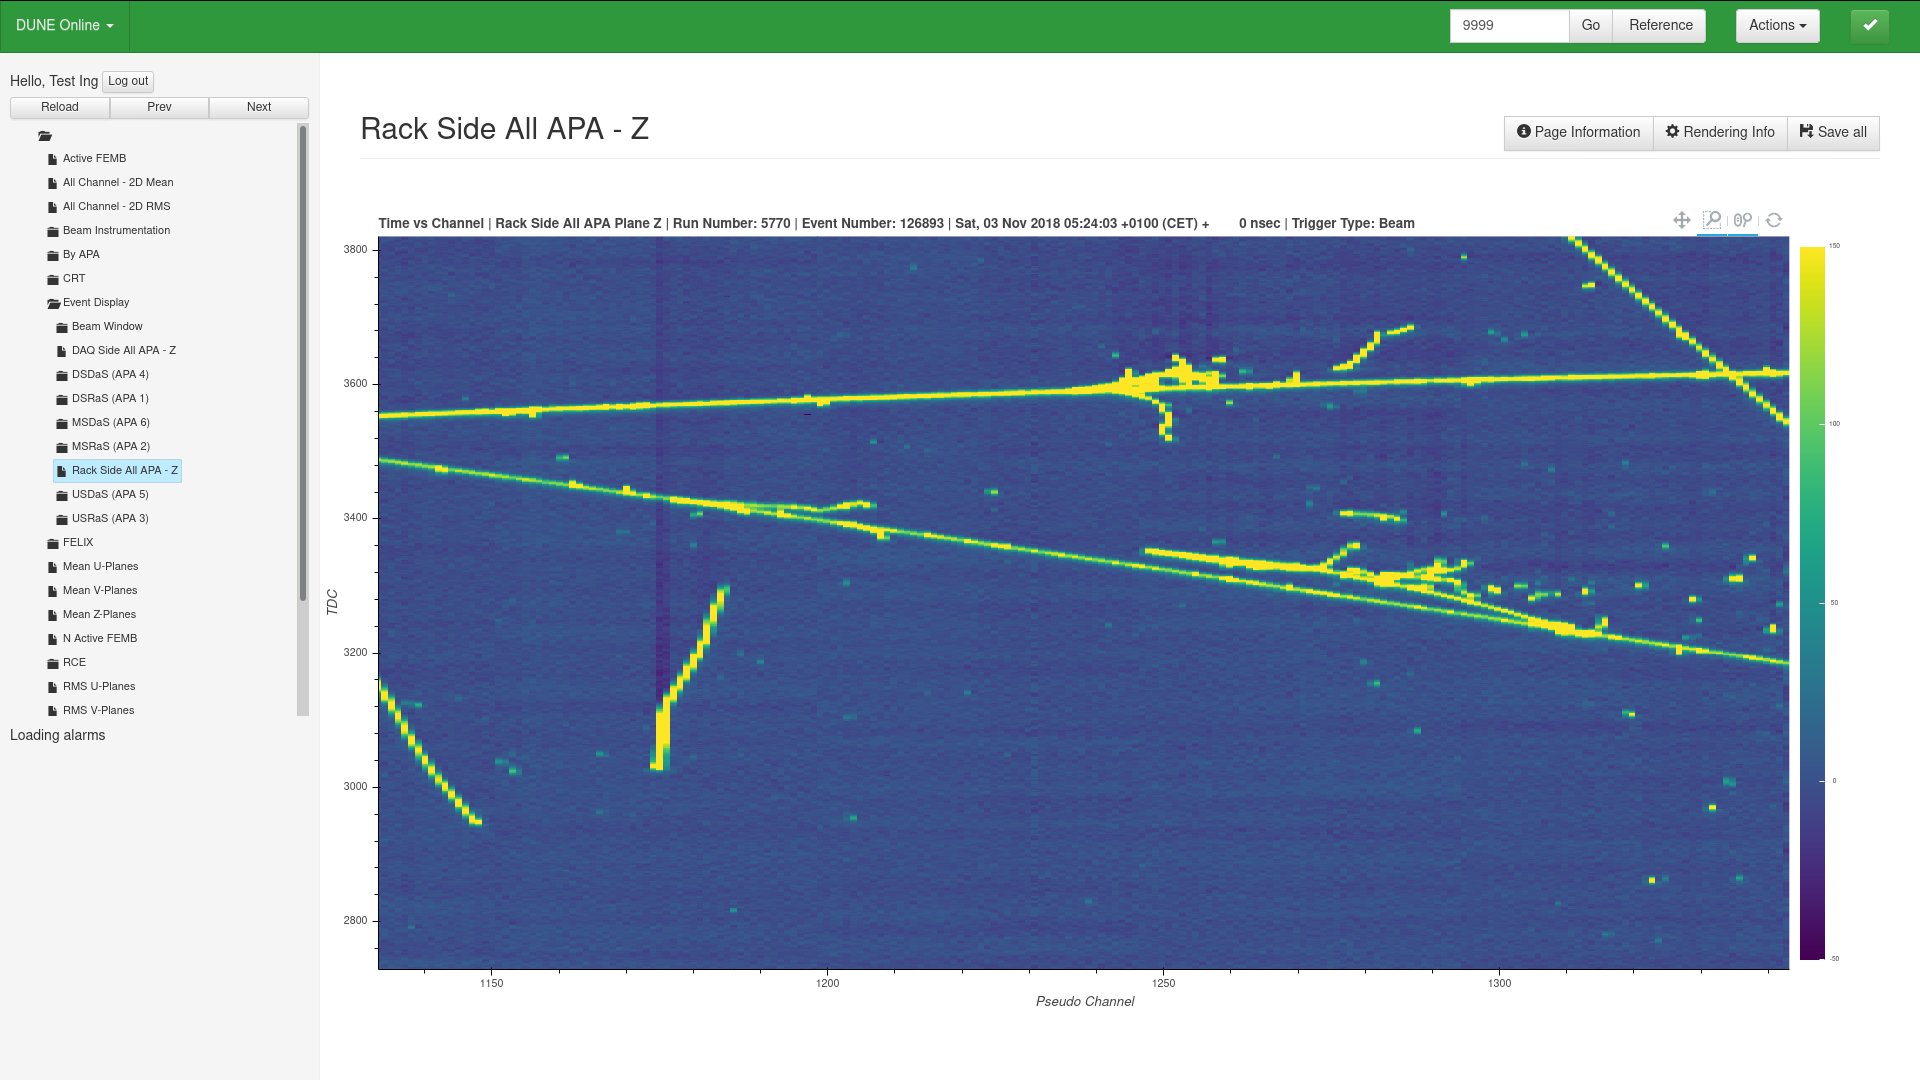
\includegraphics[width=\textwidth]{figures/zoomed_in.png}
		\caption {Zoomed region.}
		\label{fig:zoomed_in}
	\end{subfigure}

	\caption
	[Example of the dynamic binning algorithm in the \protodune{} online
	monitoring system.]
	{ Example of the dynamic binning algorithm in the \protodune{} online
	monitoring system. }
	\label{fig:dynamic_binning}

\end{figure}

The other significant modification to Monet was to modify the data handling to 
significantly improve the efficiency of data transfer to the renderer.
When Monet was first adapted for \protodune{} it was too slow to render some 
of the larger plots such as event displays, it would take minutes to render a 
single event display. By improving the efficiency of the data transfer from ROOT
to Bokeh, the rendering time was reduced to around 4 seconds per event display.
% \mccorrect{TODO: do I need to expand here or is this sufficient? Seems a little
% over the top to explain the change of algorithm.}

\bigskip

In the \protodune{} Technical Design Report \cite{Abi2017}, the proposed online
monitoring system was described as being able to \say{provide data quality 
assurance in real--time}, in practice the response time is around one minute.
During this time each set of plots will have contain data from 10 events, 
however, the event displays and TPC FFTs each contain data from one event.
\mccorrect{TODO: Should I include a discussion of possible improvements?}

% First, the OM had to wait for each data file to be closed in order to start 
% it's analysis, which means 100 events are written before the OM can start 
% looking at the data. A shared memory system was proposed in which the OM and 
% EventBuilders can simultaneously look at the data as it is coming off the 
% detector, this would reduce the latency in the OM by allowing it to analyse
% the data promptly as it is read out by the detector. Unfortunately, this system
% was never implemented during the first beam run of \protodune{}, and it remains 
% under development.
